% openany: without it, book defaults to openright, which forces every
% \part AND the \chapter* immediately following it (Introduction to Part N)
% to each start on its own fresh odd page -- wedging a blank page between
% a part's title page and its own introduction at every single boundary.
\documentclass[11pt,twoside,openany]{book}

% Essential packages
\usepackage[utf8]{inputenc}
\usepackage[T1]{fontenc}
\usepackage{geometry}
\usepackage{graphicx}
\usepackage{pdfpages}
\usepackage{hyperref}
\usepackage{bookmark}
\usepackage{fancyhdr}
\usepackage{titlesec}
\usepackage{tocloft}
\usepackage{amsmath}
\usepackage{amsfonts}
\usepackage{amssymb}
\usepackage{url}
\usepackage{cite}
\usepackage{setspace}
\usepackage{microtype}
% Professional font choice: Libertinus (modern, elegant serif with excellent math support)
\usepackage{libertinus}
\usepackage{libertinust1math}
\usepackage{textcomp}
\usepackage{xcolor}
\usepackage{enumitem}
\usepackage{mdframed}
\usepackage{fancyvrb}
\usepackage{fvextra}
\usepackage{makeidx}
\makeindex

% Enable microtypography for better text quality
\microtypesetup{protrusion=true,expansion=true,tracking=true}

% Widow and orphan control
\widowpenalty=10000
\clubpenalty=10000
\brokenpenalty=4991

% Prevent hyphenation at page breaks
\interlinepenalty=5000

% Paper summary page environment (refined academic style)
% Set via \papertoclabel{toc text}{label} immediately before \input-ing a
% paper summary; consumed below so the TOC entry and \label anchor bind to
% the fresh page \clearpage starts, not to whatever anchor preceded it.
\newcommand{\papertoclabel}[2]{%
  \gdef\CurrentPaperTocText{#1}%
  \gdef\CurrentPaperLabel{#2}%
}
\newenvironment{papersummary}[4]{% year, title, authors, one-sentence summary
  \clearpage
  \phantomsection
  \addcontentsline{toc}{subsection}{\CurrentPaperTocText}%
  \label{\CurrentPaperLabel}%
  \markright{#3 (#1)}% Set running header to "Authors (Year)"
  \thispagestyle{empty}
  \vspace*{1cm}
  \begin{center}
    {\fontsize{11}{13}\selectfont\scshape #1}\\[0.8em]
    {\fontsize{18}{22}\selectfont\bfseries #2}\\[1em]
    {\fontsize{11}{13}\selectfont\itshape #3}
  \end{center}
  \vspace{0.8em}
  \begin{center}
    \rule{0.6\textwidth}{0.4pt}
  \end{center}
  \vspace{1em}
  \noindent\textit{#4}
  \vspace{1.2em}
  \begin{mdframed}[
    linewidth=0pt,
    leftline=true,
    rightline=false,
    topline=false,
    bottomline=false,
    linecolor=black!50,
    linewidth=3pt,
    backgroundcolor=black!2,
    innertopmargin=12pt,
    innerbottommargin=12pt,
    innerrightmargin=14pt,
    innerleftmargin=14pt,
    skipabove=10pt
  ]
}{%
  \end{mdframed}
  \vfill
}

\newcommand{\summaryheading}[1]{%
  \vspace{0.5em}%
  \noindent{\scshape\bfseries #1}%
  \vspace{0.3em}%
  \par\noindent%
}

% Professional page geometry for digital reading
\geometry{
    paperwidth=7in,
    paperheight=10in,
    inner=1.15in,
    outer=0.85in,
    top=1in,
    bottom=1in,
    headheight=24pt,
    headsep=18pt,
    footskip=24pt
}

% Enhanced headers and footers: canonical twoside layout, page number on the
% outer edge of each page (left on verso, right on recto), running-head text
% toward the inner edge -- the standard convention for a book set for binding.
\pagestyle{fancy}
\fancyhf{}
\fancyhead[LE,RO]{\small\thepage}
\fancyhead[RE]{\small\textsc{\nouppercase{\leftmark}}}
\fancyhead[LO]{\small\textsc{\nouppercase{\rightmark}}}
\fancyfoot[C]{}
\renewcommand{\headrulewidth}{0.3pt}
\renewcommand{\footrulewidth}{0pt}

% Customize chapter and part marks to avoid duplication
\renewcommand{\chaptermark}[1]{\markboth{#1}{}}
\renewcommand{\partmark}[1]{\markboth{\partname\ \thepart: #1}{}}

% \chapter* never calls \chaptermark, so plain chapters (Prologue, Epilogue,
% the Revision History) would otherwise inherit whatever running head was
% last set -- e.g. "Contents" bleeding into the Prologue. \PlainChapter sets
% both marks to its own title.
\newcommand{\PlainChapter}[1]{%
  \chapter*{#1}%
  \addcontentsline{toc}{chapter}{#1}%
  \markboth{#1}{#1}%
}
% Part and appendix introduction chapters sit *within* a part: the verso
% (left) mark should keep showing the enclosing part's title, set moments
% earlier by \partmark, while the recto (right) mark narrows to the
% introduction itself -- and is overwritten again by \markright once the
% first paper begins. \markright leaves \leftmark untouched, unlike
% \markboth.
% Filed at the TOC's section level, not chapter: unlike Prologue, Epilogue,
% and the Revision History (true top-level entries, siblings of a Part),
% a part introduction is nested inside its enclosing part, and the TOC
% should show that nesting rather than list it flush with the part itself.
\newcommand{\PartIntroChapter}[1]{%
  \chapter*{#1}%
  \addcontentsline{toc}{section}{#1}%
  \markright{#1}%
}

% Chapter formatting - Springer style
\titleformat{\chapter}[display]
  {\normalfont\Large\bfseries\centering}
  {\MakeUppercase{\chaptertitlename}\ \thechapter}
  {12pt}
  {\huge\bfseries}
\titlespacing*{\chapter}{0pt}{40pt}{30pt}

% Part formatting - dramatic full-page treatment
\titleformat{\part}[display]
  {\normalfont\centering}
  {\vspace*{2cm}\rule{0.5\textwidth}{0.5pt}\\[1em]%
   {\fontsize{14}{16}\selectfont\scshape\partname}\\[0.3em]%
   {\fontsize{72}{80}\selectfont\textcolor{black!25}{\thepart}}\\[0.5em]%
   \rule{0.5\textwidth}{0.5pt}}
  {40pt}
  {\fontsize{28}{34}\selectfont\bfseries}
\titlespacing*{\part}{0pt}{0pt}{40pt}

% Section formatting
\titleformat{\section}
  {\normalfont\large\bfseries}
  {\thesection}
  {1em}
  {}
\titlespacing*{\section}{0pt}{18pt plus 4pt minus 2pt}{12pt plus 2pt minus 2pt}

% Subsection formatting
\titleformat{\subsection}
  {\normalfont\normalsize\bfseries}
  {\thesubsection}
  {1em}
  {}
\titlespacing*{\subsection}{0pt}{12pt plus 3pt minus 1pt}{8pt plus 1pt minus 1pt}

% Enhanced table of contents
\renewcommand{\cftpartfont}{\Large\bfseries}
\renewcommand{\cftchapfont}{\normalsize\bfseries}
\renewcommand{\cftsecfont}{\normalsize}
\renewcommand{\cftsubsecfont}{\small}
\renewcommand{\cftpartpagefont}{\Large\bfseries}
\renewcommand{\cftchappagefont}{\normalsize\bfseries}
\renewcommand{\cftsecpagefont}{\normalsize}
\renewcommand{\cftsubsecpagefont}{\small}
\setlength{\cftbeforepartskip}{12pt}
\setlength{\cftbeforechapskip}{6pt}
\setlength{\cftbeforesecskip}{3pt}
\setlength{\cftbeforesubsecskip}{2pt}
% Cascading indent so the TOC's nesting reads at a glance: Part (flush) <
% part introduction (section-level) < paper (subsection-level). Prologue,
% Revision History, Epilogue, and the Index stay at chapter level (flush),
% since they are not nested inside any part.
\setlength{\cftsecindent}{1.2em}
\setlength{\cftsubsecindent}{2.6em}
% None of our TOC entries use \numberline (there is no real chapter/section
% number -- the "[1943]"-style year tag is just the first word of the
% title). Without this, tocloft still reserves its book-class default
% number-column width when a long title wraps, so the second line hangs
% indented further right than the first for no reason tied to our content.
% Zeroing it makes wrapped lines fall flush with the first line instead.
\setlength{\cftpartnumwidth}{0em}
\setlength{\cftchapnumwidth}{0em}
\setlength{\cftsecnumwidth}{0em}
\setlength{\cftsubsecnumwidth}{0em}

% Dotted leaders for all TOC levels
\renewcommand{\cftpartleader}{\cftdotfill{\cftdotsep}}
\renewcommand{\cftchapleader}{\cftdotfill{\cftdotsep}}
\renewcommand{\cftsecleader}{\cftdotfill{\cftdotsep}}
\renewcommand{\cftsubsecleader}{\cftdotfill{\cftdotsep}}

% List formatting
\setlist[enumerate]{itemsep=3pt,parsep=0pt,topsep=6pt}
\setlist[itemize]{itemsep=3pt,parsep=0pt,topsep=6pt}

% A restrained, near-black ink color for cross-references: distinguishable
% from body text on close reading, but not the saturated web-hyperlink blue
% that reads as "PDF" rather than "typeset book."
\definecolor{inkblue}{RGB}{30,30,80}

% Hyperref setup - professional styling with enhanced navigation
\hypersetup{
    pdftitle={The Foundations of Large Language Models, 1943-2026},
    pdfauthor={Joe Duffy},
    pdfsubject={Artificial Intelligence, Machine Learning, Natural Language Processing},
    pdfkeywords={Large Language Models, Transformers, Neural Networks, AI, Deep Learning},
    colorlinks=true,
    linkcolor=inkblue,
    citecolor=inkblue,
    urlcolor=inkblue,
    bookmarksnumbered=true,
    bookmarksopen=true,
    pdfpagemode=UseOutlines,
    pdfdisplaydoctitle=true,
    linktoc=all
}

% Professional title page with neural network graphic
\usepackage{tikz}
\usetikzlibrary{positioning,shapes.geometric,arrows.meta,calc}

\makeatletter
\renewcommand{\maketitle}{%
  \begin{titlepage}%
    % Widen the measure for this page alone -- a title reads as a cover,
    % not a paragraph, and wants a broader column than 11pt body text.
    % Restored immediately below, before the colophon that follows.
    \newgeometry{left=0.5in, right=0.5in, top=1in, bottom=1in}%
    \let\footnotesize\small
    \let\footnoterule\relax
    \let \footnote \thanks
    % Two-zone cover in the manner of a Springer series binding: a quiet
    % white band carrying the diagram, then a solid field of the book's
    % one interior accent color carrying the title -- bold through flat,
    % confident color and clean type, not through gilding or glow.
    \begin{tikzpicture}[remember picture, overlay]
      \fill[inkblue] (current page.south west) rectangle
        ([yshift=-3.35in]current page.north east);
    \end{tikzpicture}%
    \vskip 0.6in
    \begin{center}%
      \begin{tikzpicture}[scale=0.58, transform shape]
        \tikzset{
          neuron/.style={circle, draw=inkblue, fill=white, line width=0.6pt,
                          minimum size=7pt, inner sep=1pt},
          connection/.style={draw=inkblue!40, line width=0.4pt}
        }
        % Input layer
        \foreach \y in {1,2,3,4} {
          \node[neuron] (I\y) at (0,\y) {};
        }
        % Hidden layers
        \foreach \y in {1,2,3,4,5} {
          \node[neuron] (H1\y) at (2,\y+0.5) {};
        }
        \foreach \y in {1,2,3,4,5,6} {
          \node[neuron] (H2\y) at (4,\y+0.25) {};
        }
        \foreach \y in {1,2,3,4} {
          \node[neuron] (H3\y) at (6,\y+0.5) {};
        }
        % Output layer
        \foreach \y in {1,2,3} {
          \node[neuron] (O\y) at (8,\y+1) {};
        }
        % Connections (subset for visual clarity)
        \foreach \i in {1,2,3,4} {
          \foreach \j in {1,3,5} {
            \draw[connection] (I\i) -- (H1\j);
          }
        }
        \foreach \i in {1,3,5} {
          \foreach \j in {2,4,6} {
            \draw[connection] (H1\i) -- (H2\j);
          }
        }
        \foreach \i in {2,4,6} {
          \foreach \j in {1,3} {
            \draw[connection] (H2\i) -- (H3\j);
          }
        }
        \foreach \i in {1,3} {
          \foreach \j in {1,2,3} {
            \draw[connection] (H3\i) -- (O\j);
          }
        }
      \end{tikzpicture}\\[65pt]
      % Two voices only, to keep the page from reading as a ransom note:
      % the title is the sole bold, capitalized, letterspaced line; every
      % other line below shares one plain, unbolded style, distinguished
      % from the title by weight and case alone rather than by switching
      % sizes and treatments line to line.
      \color{white}%
      {\fontsize{23}{27}\selectfont\bfseries\textls[70]{\MakeUppercase{The Foundations of}}}\\[12pt]
      {\fontsize{30}{35}\selectfont\bfseries\textls[70]{\MakeUppercase{Large Language Models}}}\\[22pt]
      \rule{2.6cm}{0.6pt}\\[18pt]
      {\large\itshape 1943 -- 2026 \textperiodcentered\ Second Edition}
      \vfill
    \end{center}\par
    \@thanks
    \vfil\null
    \restoregeometry
  \end{titlepage}%
  \setcounter{footnote}{0}%
  \global\let\thanks\relax
  \global\let\maketitle\relax
  \global\let\@thanks\@empty
  \global\let\@author\@empty
  \global\let\@date\@empty
  \global\let\@title\@empty
  \global\let\title\relax
  \global\let\author\relax
  \global\let\date\relax
  \global\let\and\relax
}
\makeatother

% Special page styles
\fancypagestyle{plain}{%
  \fancyhf{}%
  \fancyfoot[C]{\small\thepage}%
  \renewcommand{\headrulewidth}{0pt}%
  \renewcommand{\footrulewidth}{0pt}%
}

% Clean page style for included PDFs (no headers/footers)
\fancypagestyle{empty}{%
  \fancyhf{}%
  \renewcommand{\headrulewidth}{0pt}%
  \renewcommand{\footrulewidth}{0pt}%
}

% Line spacing: single, dense setting in the manner of a typeset mathematics
% monograph rather than a manuscript draft. (Deliberately placed after all
% packages, including tikz, have finished loading.)
\singlespacing

\begin{document}

% Front matter
\frontmatter
\maketitle

% Copyright / colophon page (verso of the title page)
\clearpage
\thispagestyle{empty}
\vspace*{\fill}
\begin{center}
\footnotesize
\textit{The Foundations of Large Language Models, 1943--2026}\\[6pt]
Copyright \textcopyright\ 2026 Joe Duffy\\[12pt]
\begin{minipage}{0.72\textwidth}
\centering
This work is licensed under the Creative Commons
Attribution-NonCommercial-ShareAlike 4.0 International License
(CC~BY-NC-SA~4.0). To view a copy of this license, visit
\url{https://creativecommons.org/licenses/by-nc-sa/4.0/}.

\vspace{8pt}
The individual research papers reproduced in this collection retain
their original copyrights and licenses as held by their respective
authors and publishers. This license applies only to the original
prose, commentary, and organization of this volume.
\end{minipage}\\[18pt]
Second Edition \textperiodcentered\ August 1, 2026\\[4pt]
\texttt{joeduffy@acm.org}
\end{center}
\vspace*{\fill}


% Frontispiece: microGPT — the complete algorithm on one page
\input{content/microgpt}

% Table of Contents
\phantomsection
\markboth{Contents}{Contents}
\setcounter{tocdepth}{2}  % Show parts, chapters, and subsections
\tableofcontents

% Revision History
\PlainChapter{Revision History}

\noindent\textbf{First Edition --- February 18, 2026.}\quad 71 papers in seven chronological
parts and three appendices, spanning 1943--2025.

\medskip
\noindent\textbf{Second Edition --- August 1, 2026.}\quad Added Part VIII, \emph{Reasoning and
the Open Frontier} (2024--2026): GRPO, multi-token prediction, auxiliary-loss-free load
balancing, T\"ulu~3 and verifiable rewards, Muon, Kimi Delta Attention, and LatentMoE, with
DeepSeek-R1 moved in from the former system-reports appendix. Added knowledge distillation,
AdamW, RMSNorm, speculative decoding, and LLM-QAT to Parts III--VII, and extended the agents
appendix through the agentic reinforcement-learning era with Reflexion, SWE-agent, and
Search-R1.

Adopted a stricter selection policy: the book now embeds foundational technique papers only,
never model or system reports. This removed the former system-reports appendix (GPT-4,
Gemini~1.5, DeepSeek-V3, o1, GPT-5) along with Llama~2 and Mixtral, whose lasting techniques are
documented by the method papers that introduced them, and corrected the LLaMA facsimile, which
had been a duplicate of Llama~2.

Rewrote the prologue and epilogue as a matched pair. The prologue's argument now carries forward
through preference optimization, verifiable rewards, and trained agency rather than stopping at
pretraining-era scale; the epilogue opens by returning to the prologue's central question, adds a
section on the reliability of long-horizon agents, and closes on a specific, still-open question
about reasoning-chain faithfulness.

\medskip
Also reset the book's typography toward the standard of a bound mathematics monograph ---
twoside layout, canonical running heads, a back-of-book index --- and corrected a number of
structural defects along the way, from mismatched table-of-contents anchors and a frozen running
head to several stray blank pages and a title page that briefly overflowed onto a second sheet.


% Prologue
\input{content/prologue}

% Main content
\mainmatter

% Part I: Neural Beginnings & Learning Mechanisms (1943–1990)
\part[Neural Beginnings \& Learning Mechanisms]{Neural Beginnings \& Learning Mechanisms\texorpdfstring{\\}{, }1943--1990}
\input{content/part1-chapter}

% Part II: Sequence Models & Word Embeddings (1997–2013)
\part[Sequence Models \& Word Embeddings]{Sequence Models \& Word Embeddings\texorpdfstring{\\}{, }1997--2013}
% Part II: Sequence Models & Word Embeddings (1997–2013)

\input{content/part2-intro}

% Papers follow
% Part II Papers: Sequence Models & Word Embeddings (1997–2013)

\papertoclabel{[1997] Long Short-Term Memory (Hochreiter \& Schmidhuber)}{paper:hochreiter-schmidhuber-1997}{\index{Hochreiter, Sepp}\index{Schmidhuber, J\"urgen}}
\input{content/summary-hochreiter-schmidhuber-1997}
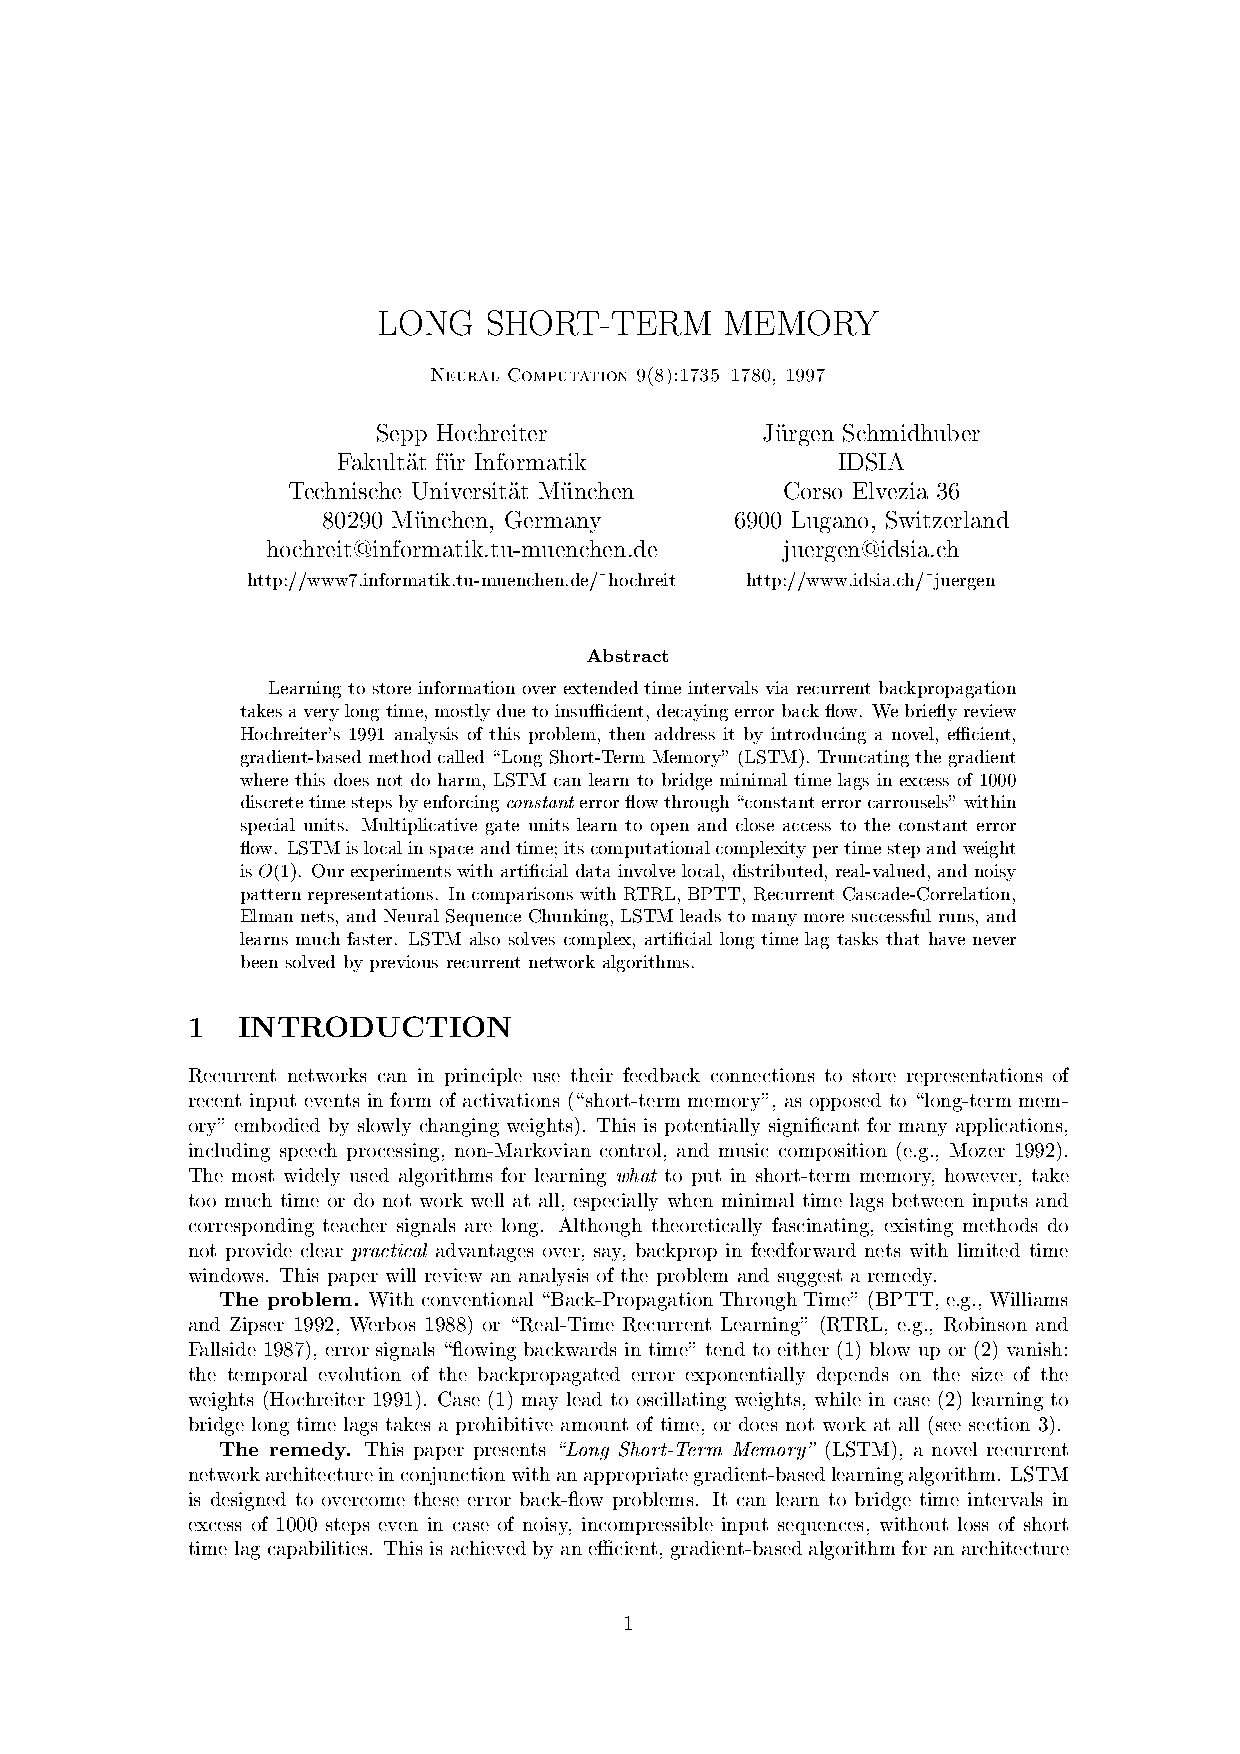
\includepdf[pages=-,pagecommand={\thispagestyle{empty}}]{pdfs/hochreiter-schmidhuber-1997.pdf}

\papertoclabel{[2003] A Neural Probabilistic Language Model (Bengio et al.)}{paper:bengio-2003}{\index{Bengio, Yoshua}\index{Ducharme, R\'ejean}\index{Vincent, Pascal}\index{Jauvin, Christian}}
\input{content/summary-bengio-2003}
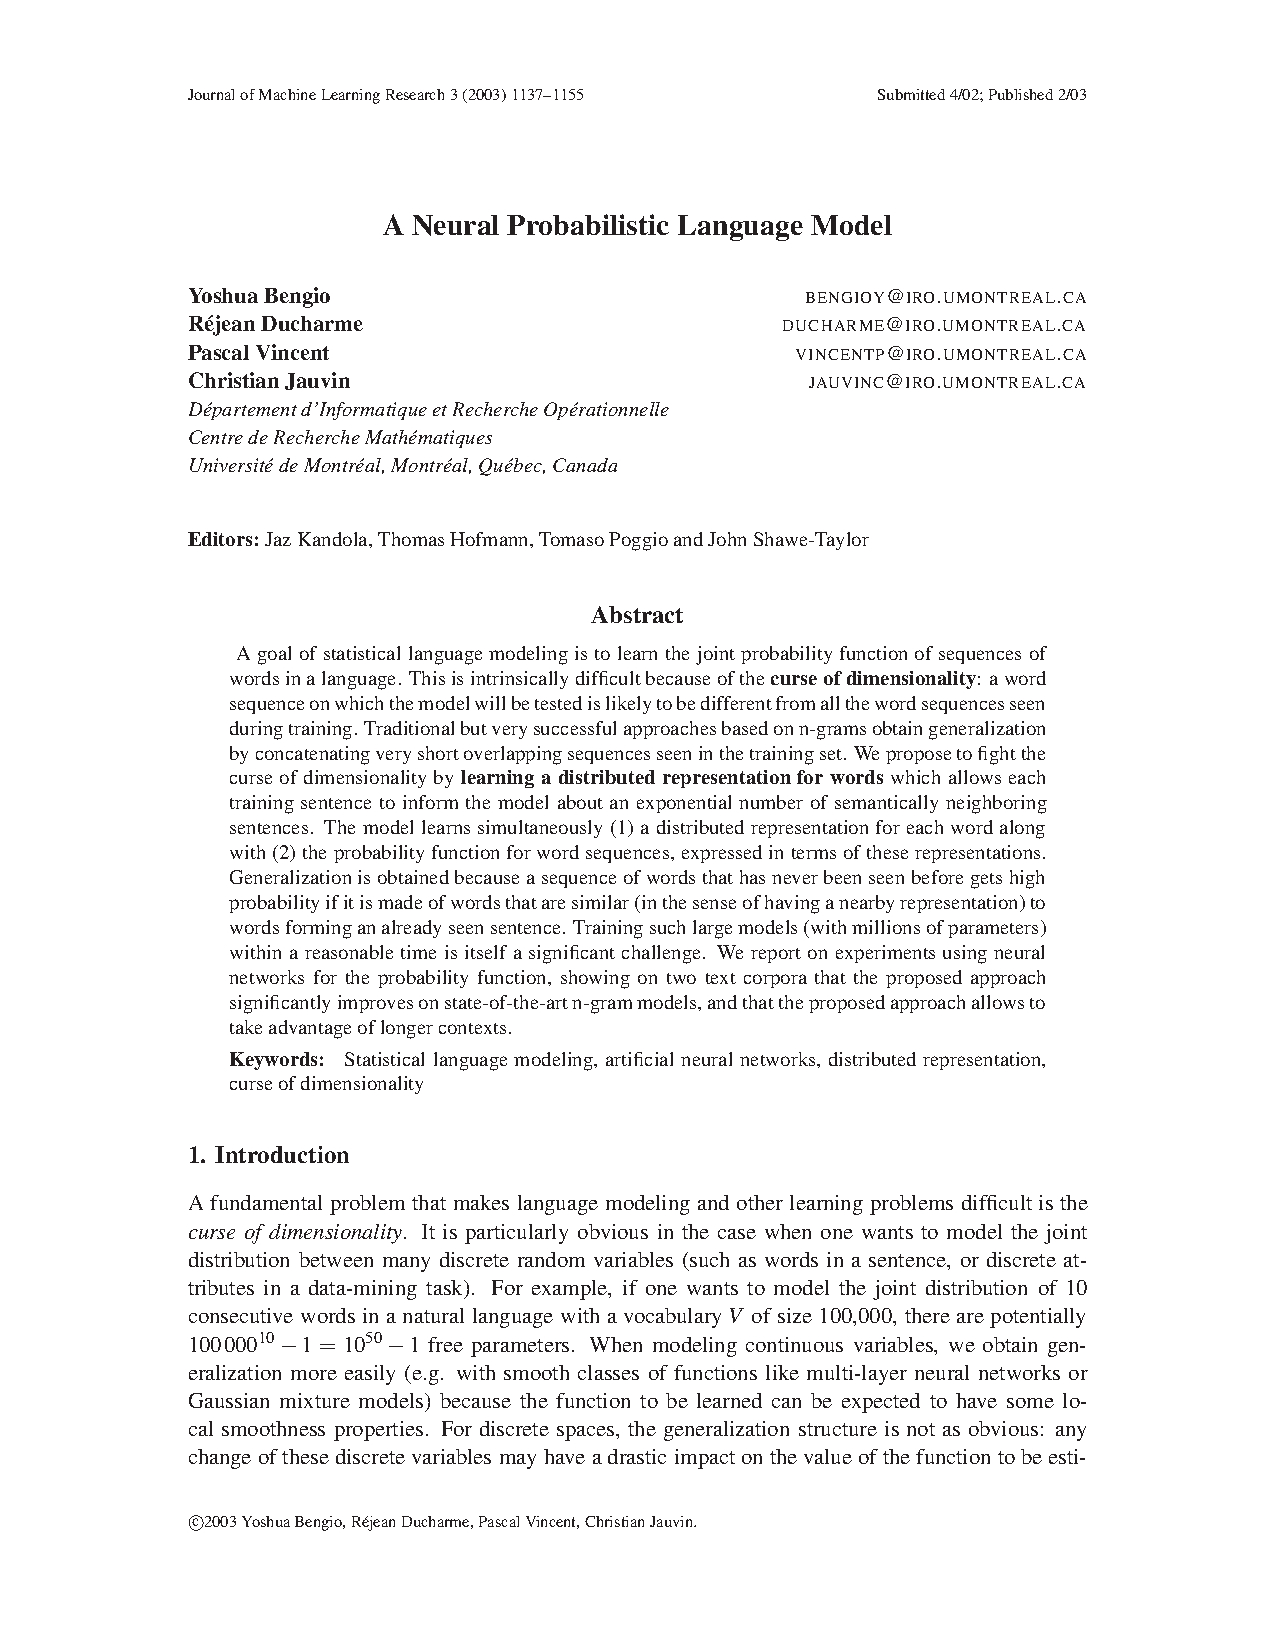
\includepdf[pages=-,pagecommand={\thispagestyle{empty}}]{pdfs/bengio-2003.pdf}

\papertoclabel{[2010] Understanding the Difficulty of Training Deep Feedforward Neural Networks (Glorot \& Bengio)}{paper:glorot-bengio-2010}{\index{Glorot, Xavier}\index{Bengio, Yoshua}}
\input{content/summary-glorot-bengio-2010}
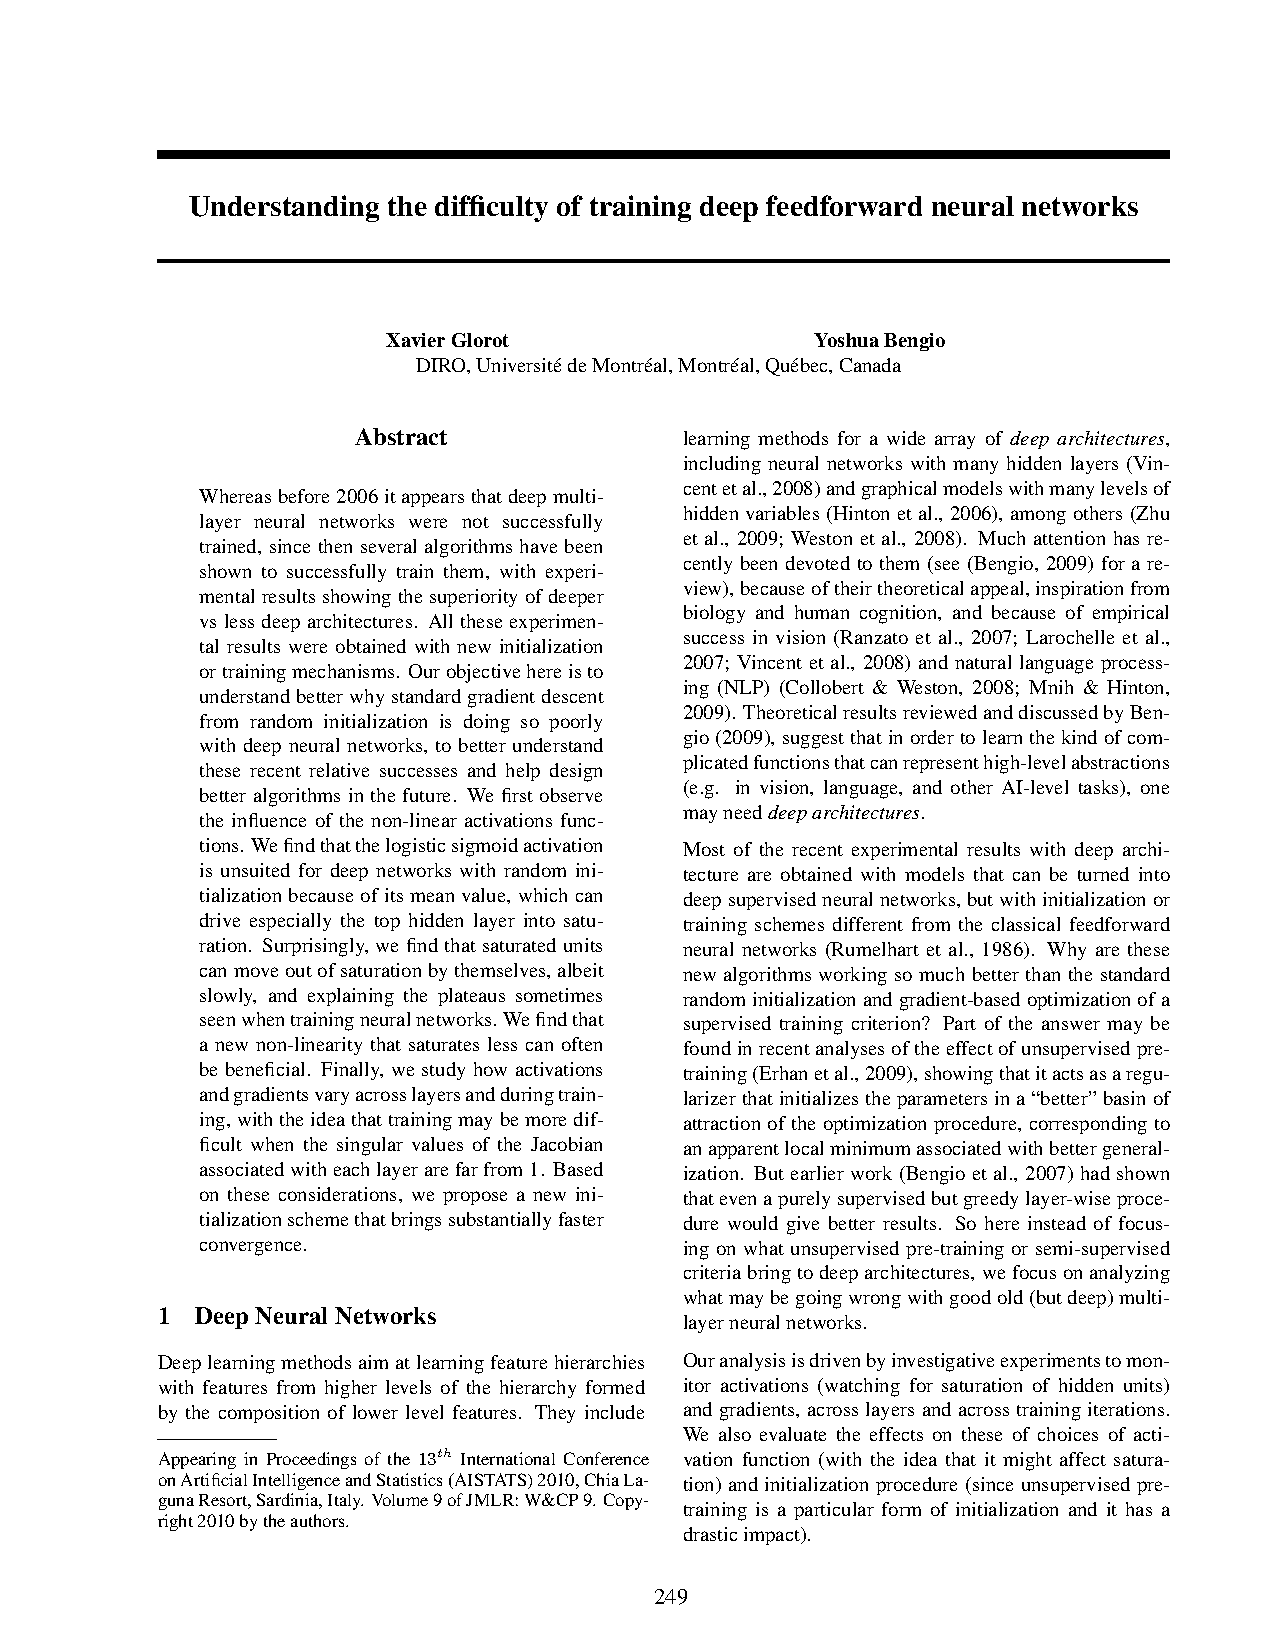
\includepdf[pages=-,pagecommand={\thispagestyle{empty}}]{pdfs/glorot-bengio-2010.pdf}

\papertoclabel{[2011] Natural Language Processing (Almost) from Scratch (Collobert et al.)}{paper:collobert-weston-2011}{\index{Collobert, Ronan}\index{Weston, Jason}\index{Bottou, L\'{e}on}\index{Karlen, Michael}\index{Kavukcuoglu, Koray}\index{Kuksa, Pavel}}
\input{content/summary-collobert-weston-2011}
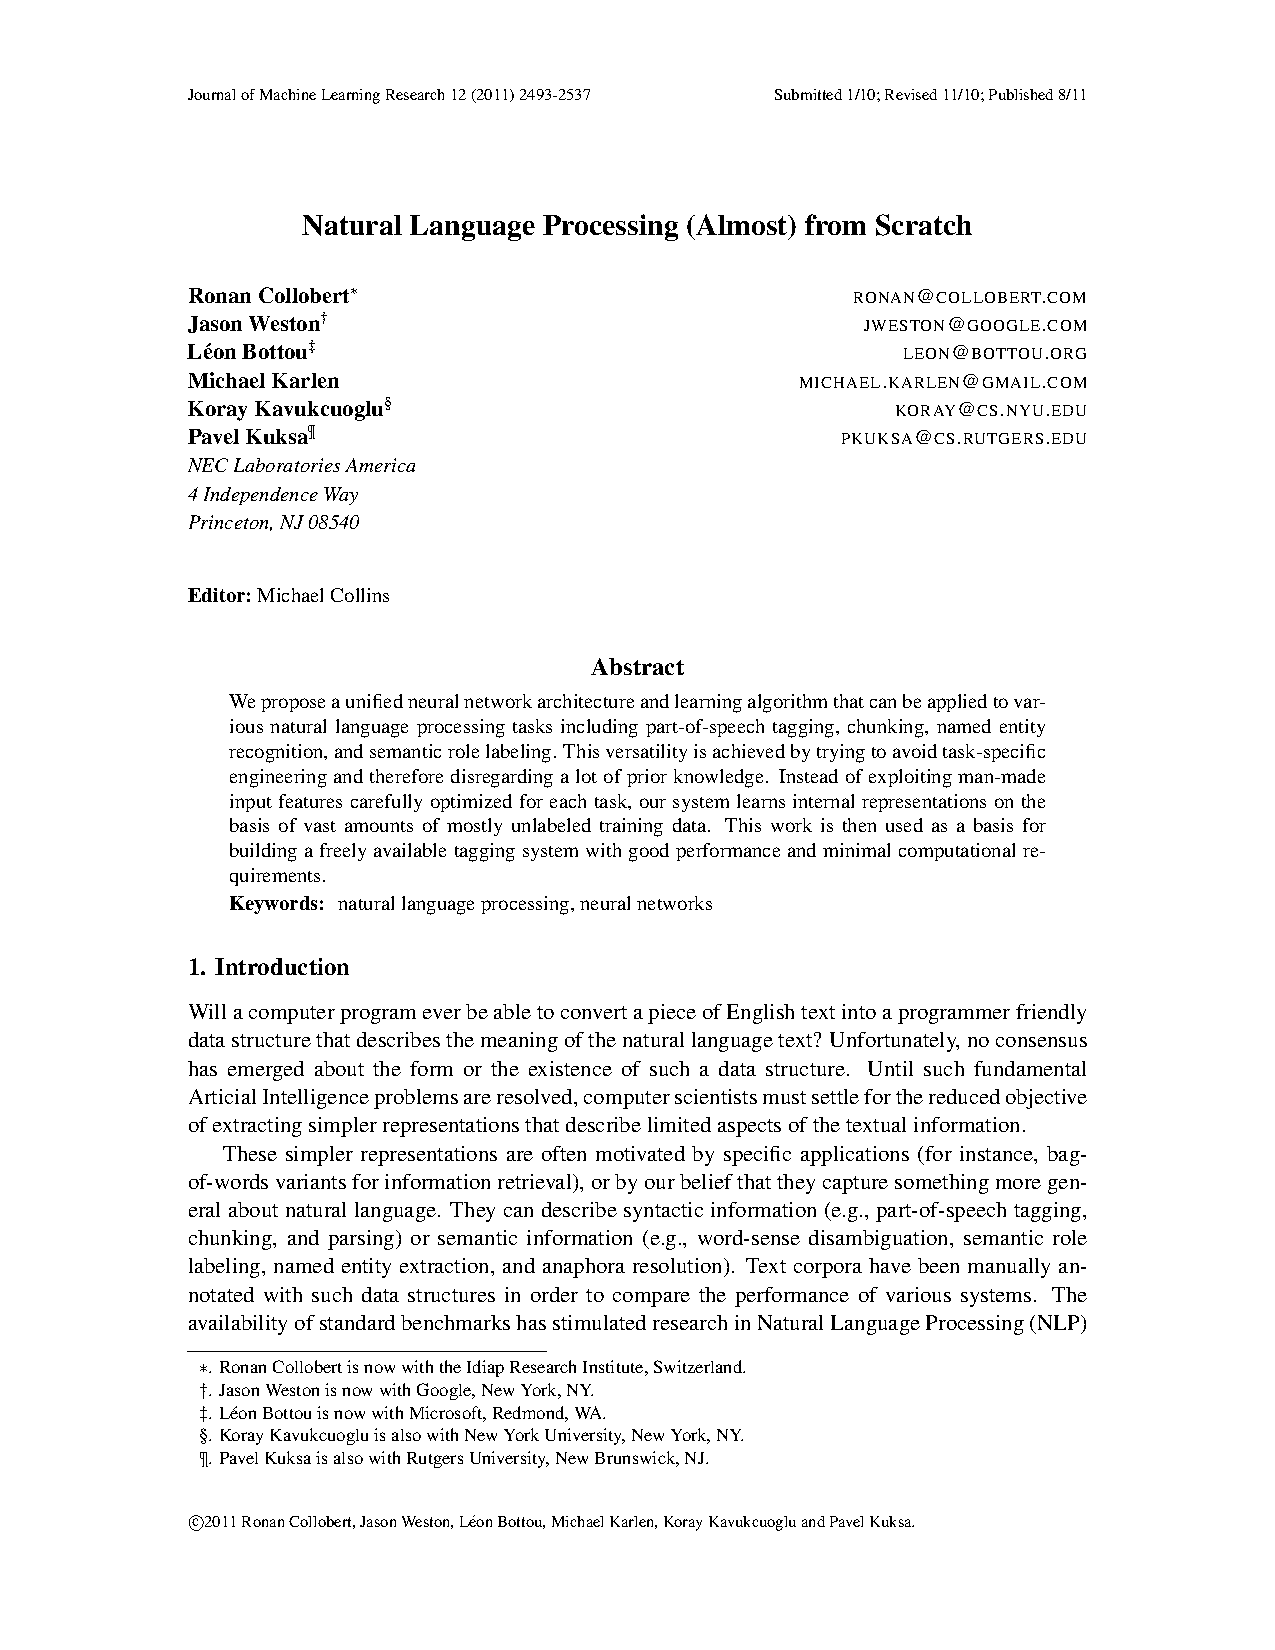
\includepdf[pages=-,pagecommand={\thispagestyle{empty}}]{pdfs/collobert-weston-2011.pdf}

\papertoclabel{[2013] Efficient Estimation of Word Representations in Vector Space (Mikolov et al.)}{paper:mikolov-2013}{\index{Mikolov, Tomas}\index{Chen, Kai}\index{Corrado, Greg}\index{Dean, Jeff}}
\input{content/summary-mikolov-2013}
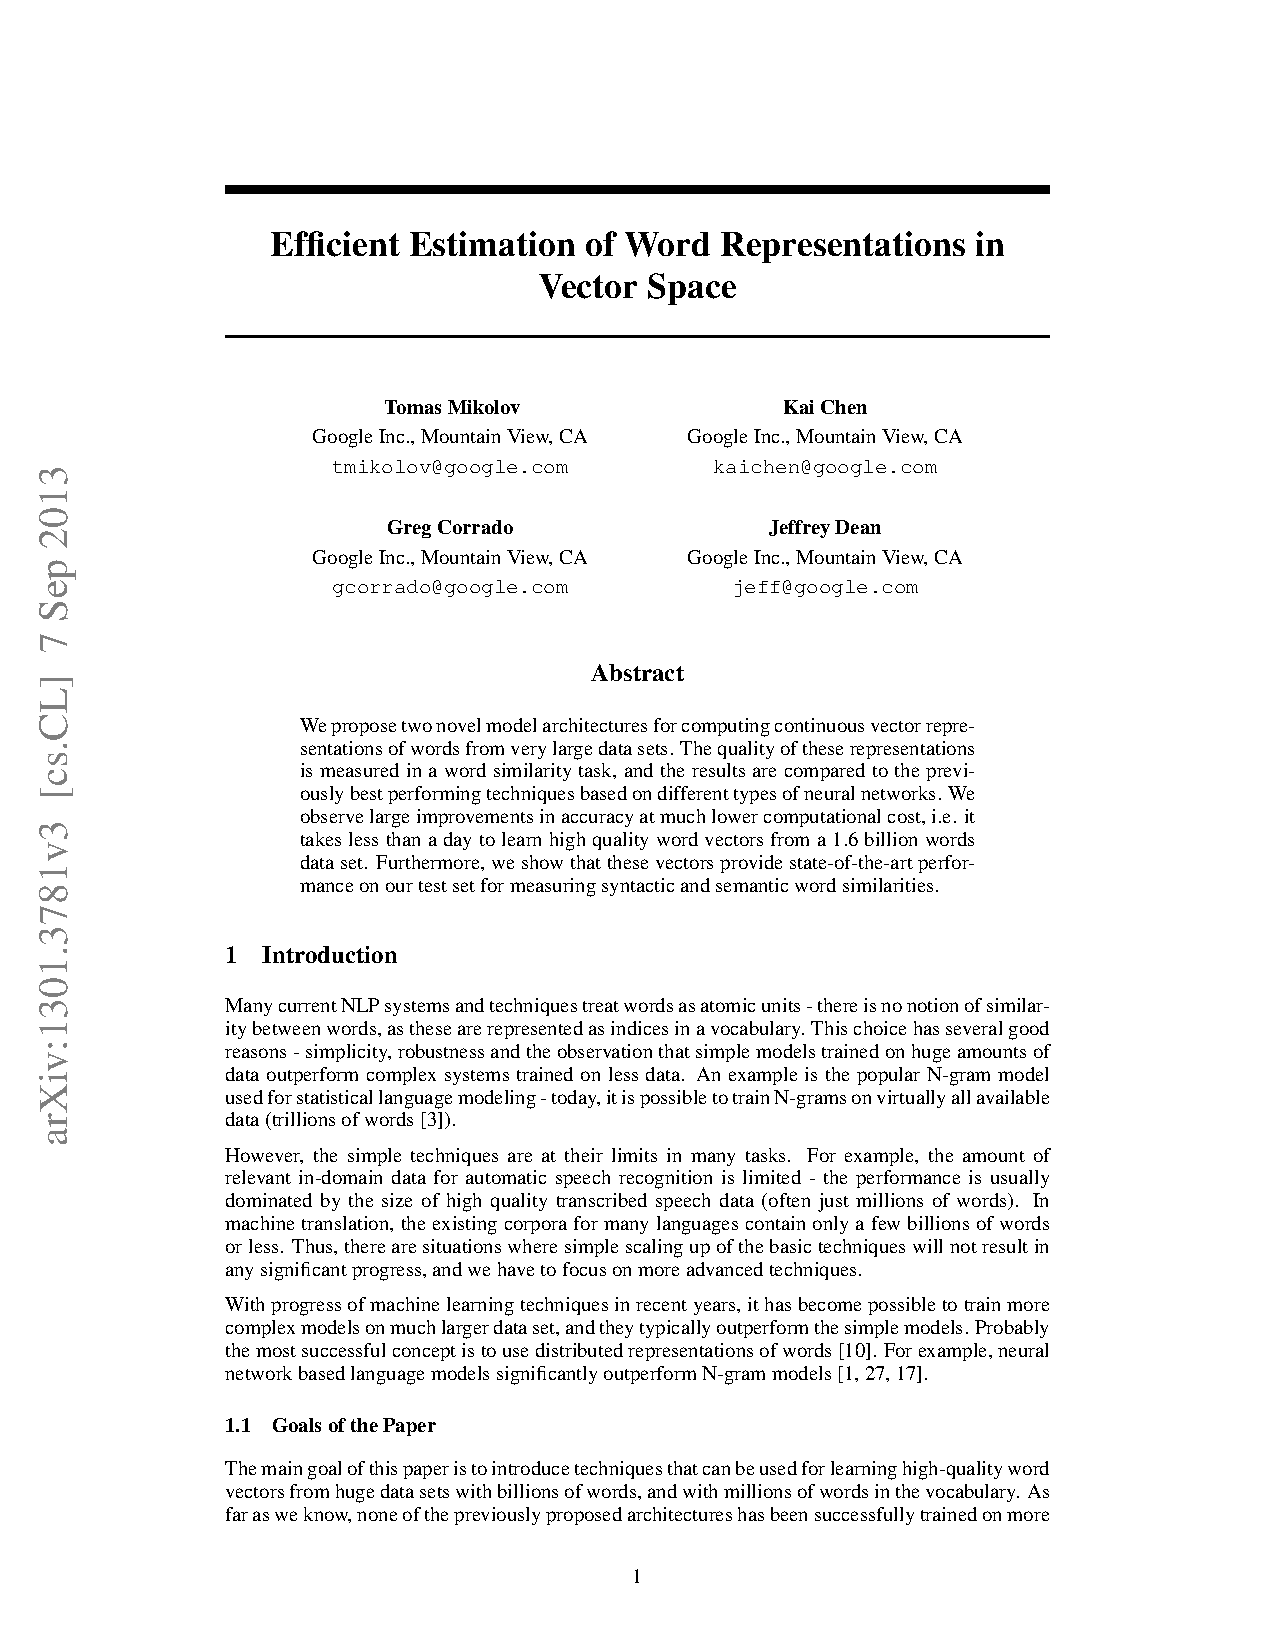
\includepdf[pages=-,pagecommand={\thispagestyle{empty}}]{pdfs/mikolov-2013.pdf}

\papertoclabel{[2013] Generating Sequences With Recurrent Neural Networks (Graves)}{paper:graves-2013}{\index{Graves, Alex}}
\input{content/summary-graves-2013}
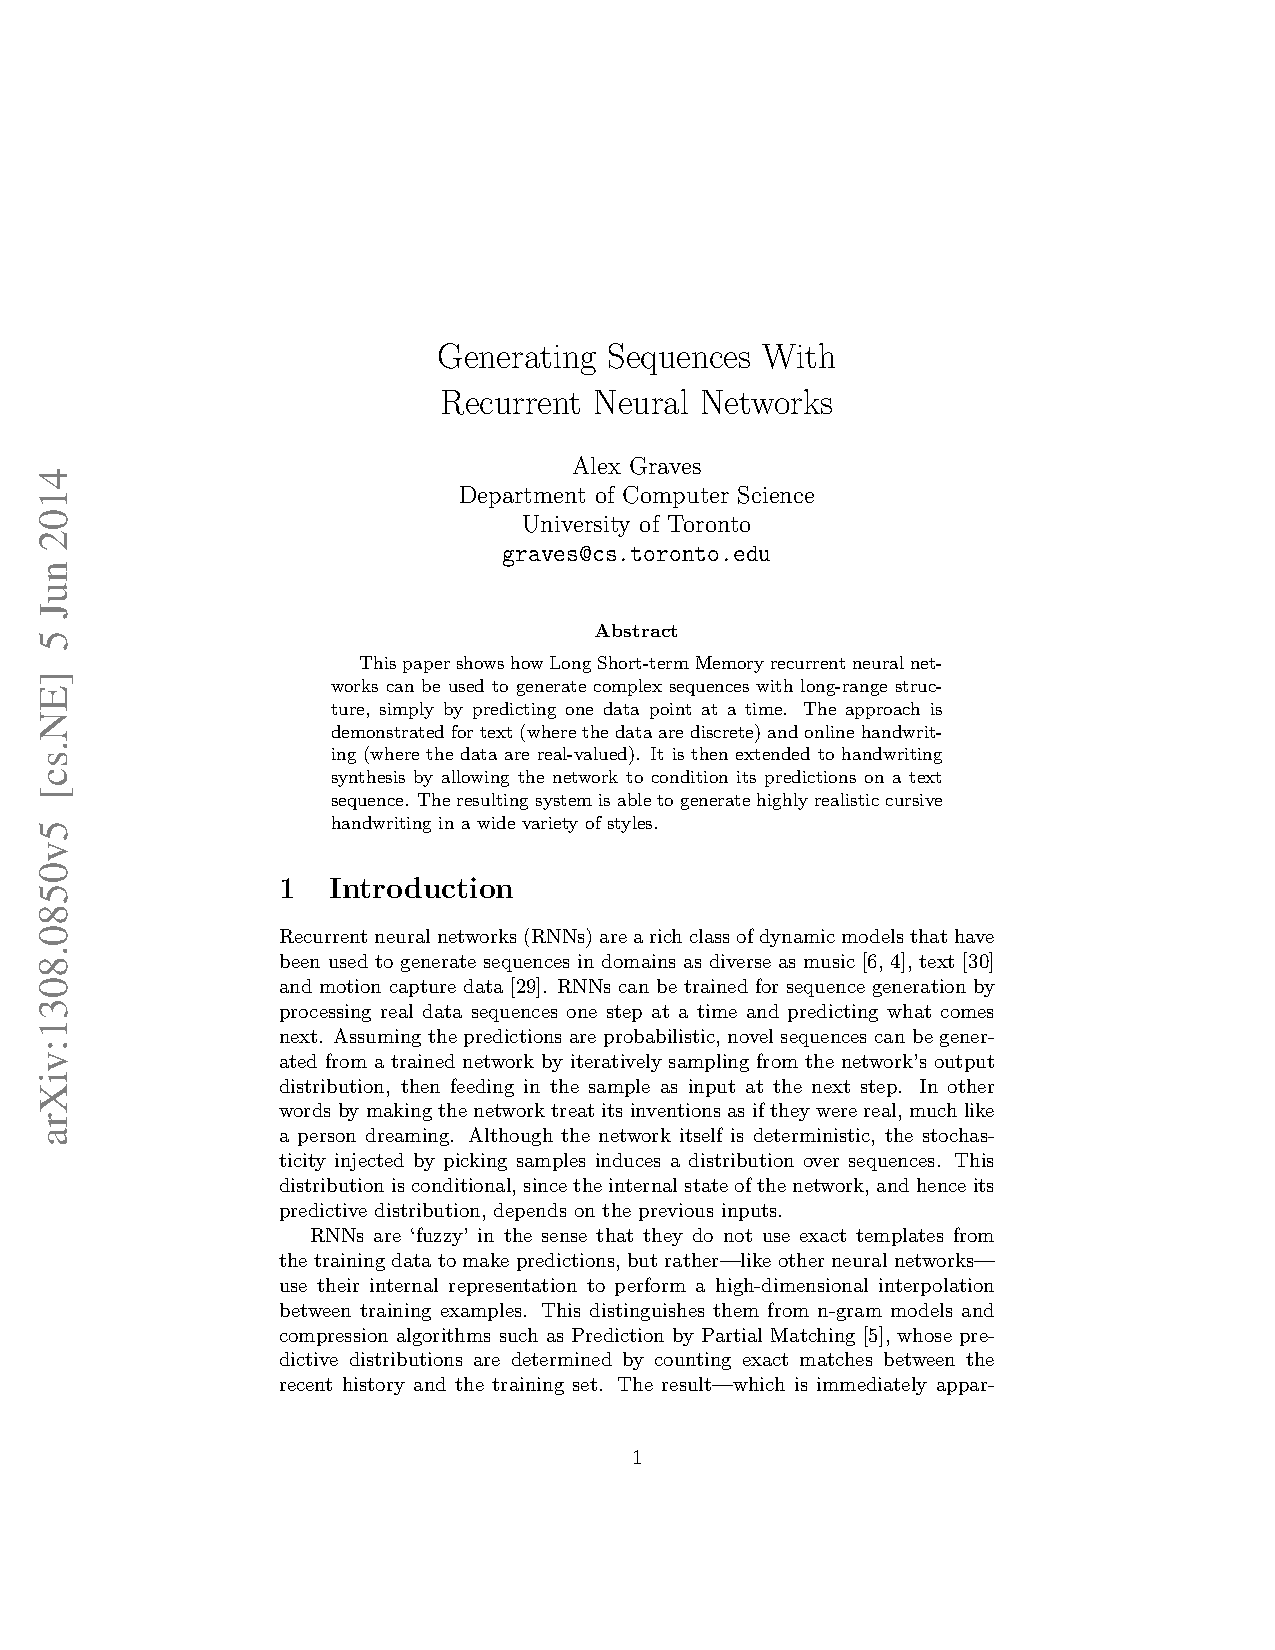
\includepdf[pages=-,pagecommand={\thispagestyle{empty}}]{pdfs/graves-2013.pdf}



% Part III: Deep Learning & Attention (2012–2015)
\part[Deep Learning \& Attention]{Deep Learning \& Attention\texorpdfstring{\\}{, }2012--2015}
\input{content/part3-chapter-new}

% Part IV: The Transformer Era and Pretraining Revolution (2016–2019)
\part[The Transformer Era and Pretraining Revolution]{The Transformer Era and Pretraining Revolution\texorpdfstring{\\}{, }2016--2019}
% Part IV: The Transformer Era and Pretraining Revolution (2016–2019)

\input{content/part4-intro}

% Papers follow
% Part IV Papers: The Transformer Era and Pretraining Revolution (2016–2019)

\papertoclabel{[2016] Layer Normalization (Ba, Kiros \& Hinton)}{paper:ba-2016}{\index{Ba, Jimmy Lei}\index{Kiros, Jamie Ryan}\index{Hinton, Geoffrey}}
\input{content/summary-ba-2016}
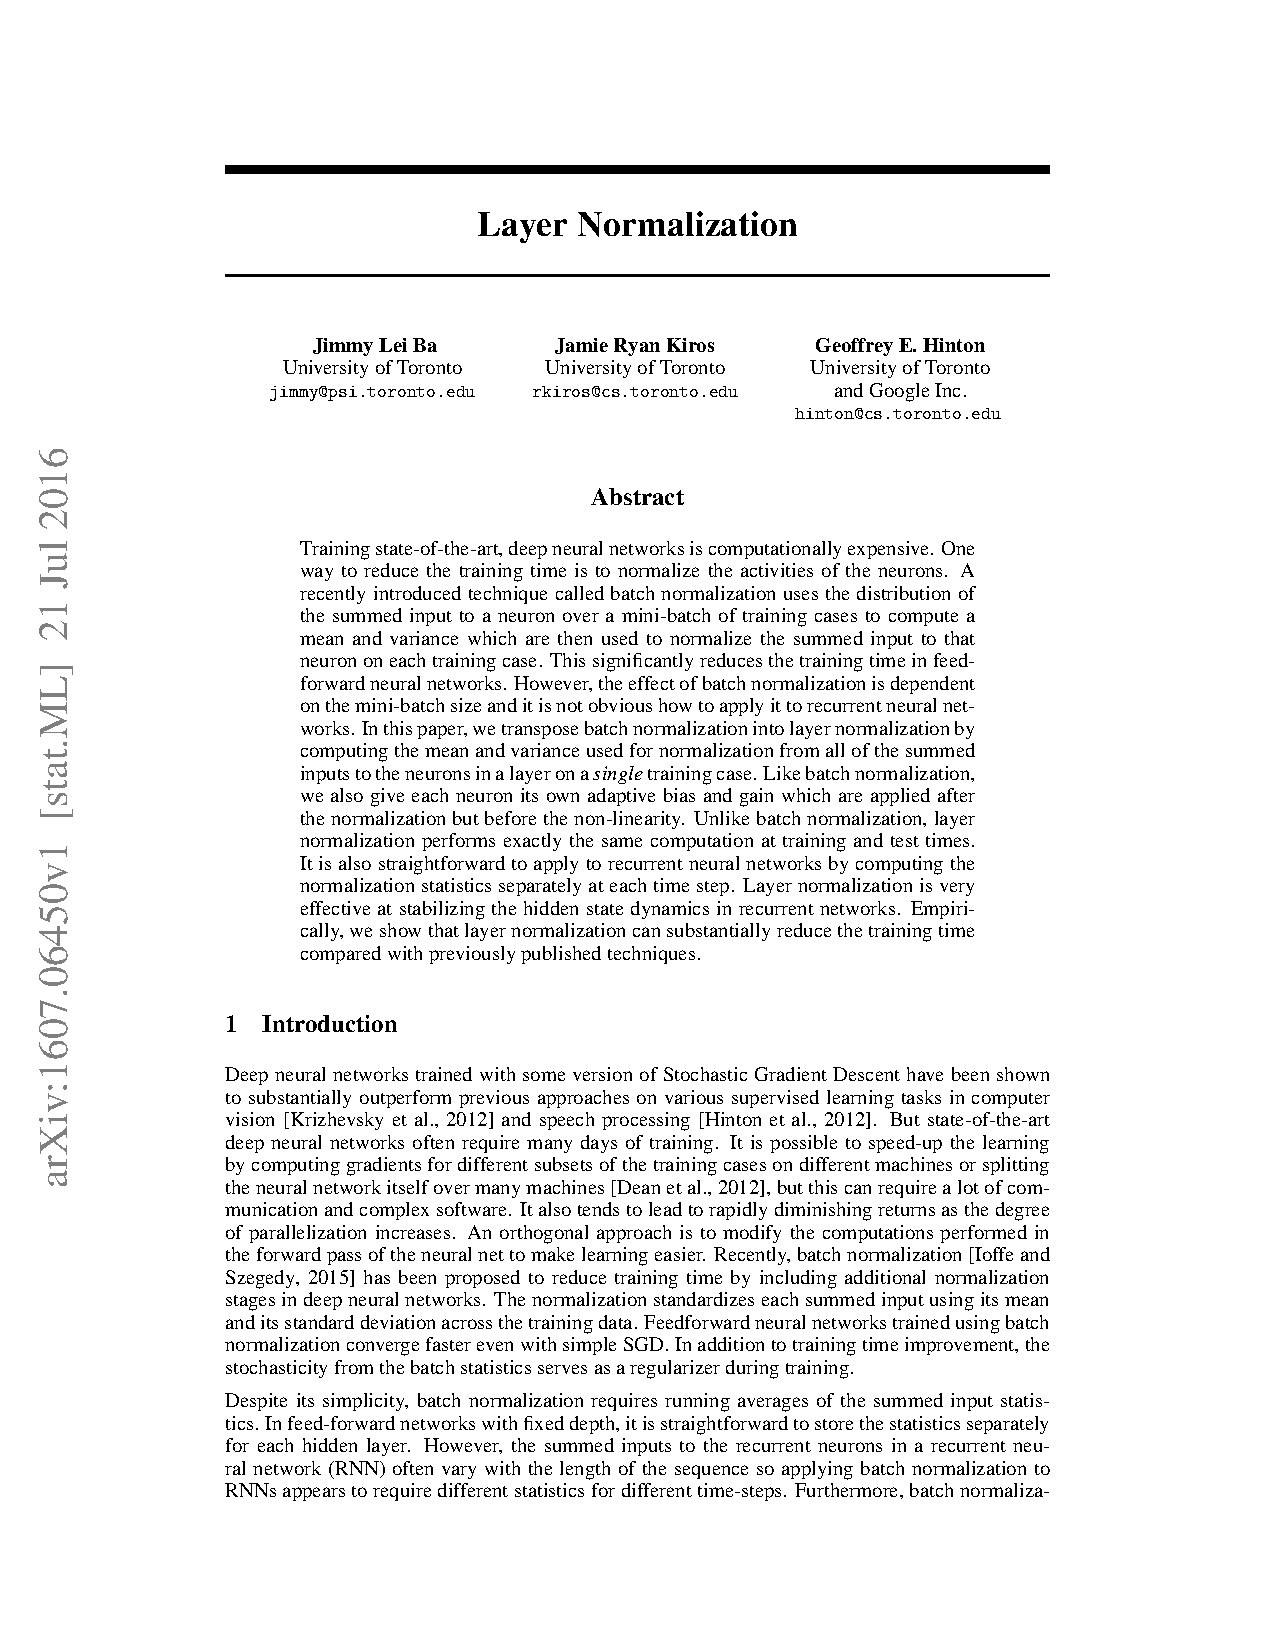
\includepdf[pages=-,pagecommand={\thispagestyle{empty}}]{pdfs/ba-2016-layernorm.pdf}

\papertoclabel{[2017] Attention Is All You Need (Vaswani et al.)}{paper:vaswani-2017}{\index{Vaswani, Ashish}\index{Shazeer, Noam}\index{Parmar, Niki}\index{Uszkoreit, Jakob}\index{Jones, Llion}\index{Gomez, Aidan N.}\index{Kaiser, Lukasz}\index{Polosukhin, Illia}}
\input{content/summary-vaswani-2017}
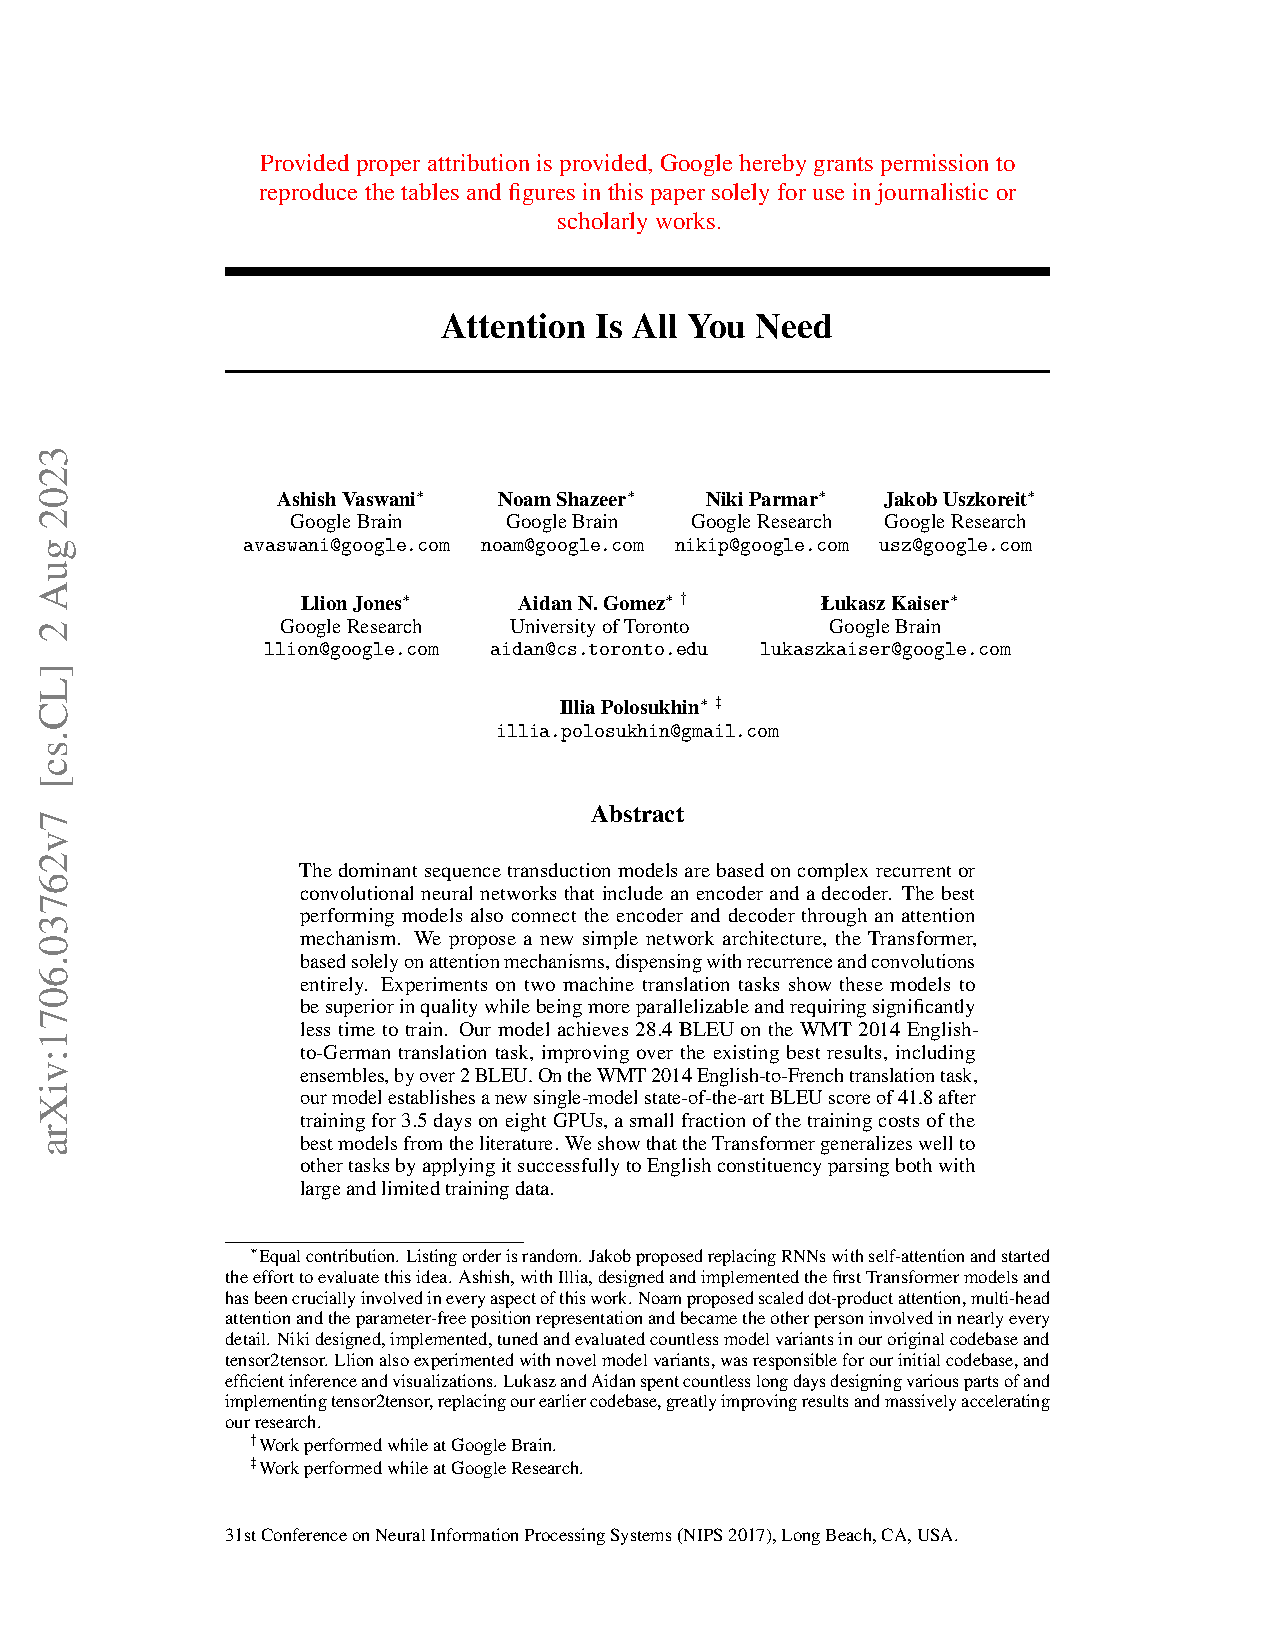
\includepdf[pages=-,pagecommand={\thispagestyle{empty}}]{pdfs/vaswani-2017.pdf}

\papertoclabel{[2017] Outrageously Large Neural Networks: The Sparsely-Gated Mixture-of-Experts Layer (Shazeer et al.)}{paper:shazeer-2017-moe}{\index{Shazeer, Noam}\index{Mirhoseini, Azalia}\index{Maziarz, Krzysztof}\index{Davis, Andy}\index{Le, Quoc V.}\index{Hinton, Geoffrey}\index{Dean, Jeff}}
\input{content/summary-shazeer-2017-moe}
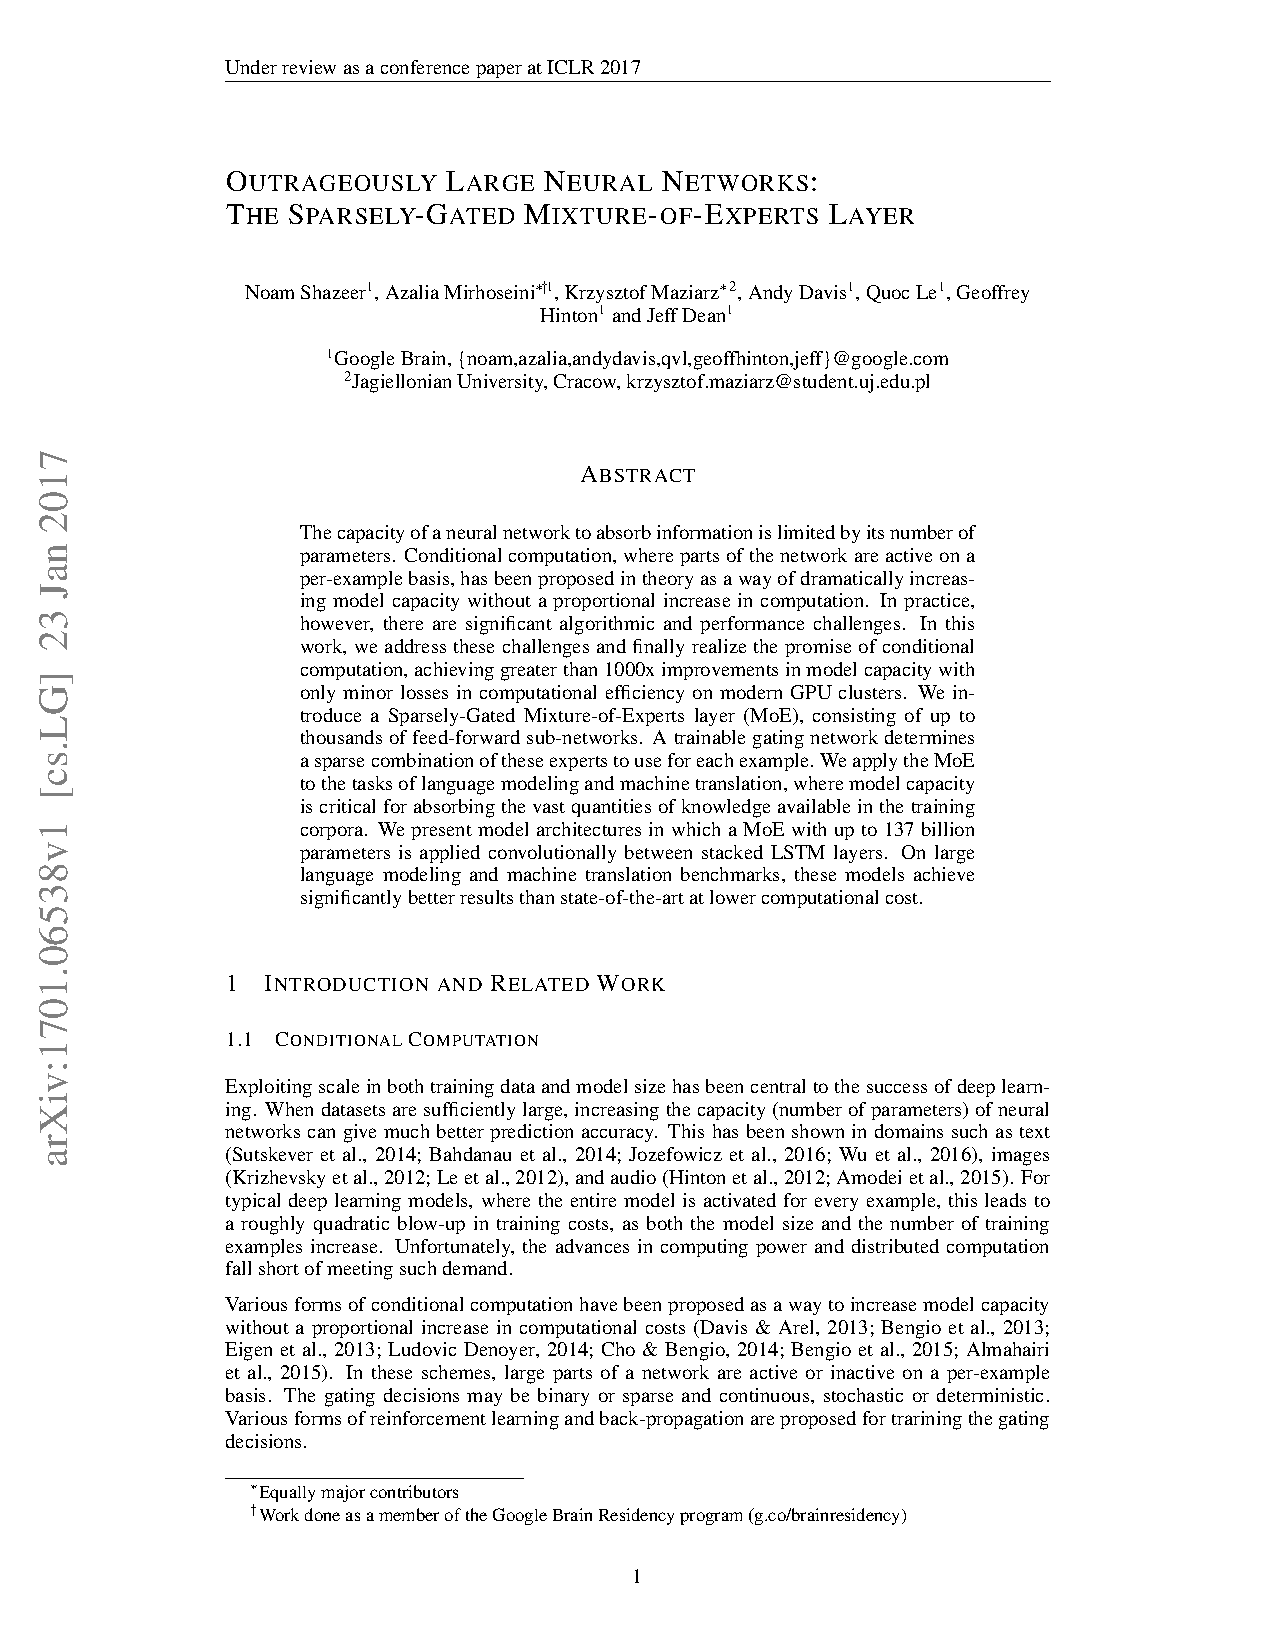
\includepdf[pages=-,pagecommand={\thispagestyle{empty}}]{pdfs/shazeer-2017-moe.pdf}

\papertoclabel{[2017] Proximal Policy Optimization Algorithms (Schulman et al.)}{paper:schulman-2017-ppo}{\index{Schulman, John}\index{Wolski, Filip}\index{Dhariwal, Prafulla}\index{Radford, Alec}\index{Klimov, Oleg}}
% Paper Summary: Proximal Policy Optimization Algorithms (Schulman et al., 2017)

\begin{papersummary}{2017}{Proximal Policy Optimization Algorithms}{John Schulman, Filip Wolski, Prafulla Dhariwal, Alec Radford, Oleg Klimov}{PPO introduced a simple yet effective policy gradient method that constrains policy updates to improve training stability, becoming the standard RL algorithm for fine-tuning large language models with human feedback.}

\summaryheading{Key Ideas}
PPO addresses the instability of policy gradient methods by constraining policy updates to remain close to the previous policy. The algorithm uses a clipped surrogate objective that prevents excessively large policy updates, maintaining training stability while achieving strong performance. PPO is simpler to implement and tune than previous methods like TRPO while matching or exceeding their performance. The algorithm balances exploration and exploitation through its conservative update strategy, making it reliable across diverse environments and tasks.

\summaryheading{Follow-on Works}
The contemporaneous preference-learning work of \hyperref[paper:christiano-2017-rlhf]{Christiano et al.\ (2017)} used TRPO and A2C; \hyperref[paper:ziegler-2019]{Ziegler et al.\ (2019)} first paired PPO with a learned reward model on language models, and \hyperref[paper:ouyang-2022]{InstructGPT (Ouyang et al., 2022)} was the first large-scale PPO-based RLHF, fine-tuning GPT-3 against human preferences under a KL penalty to the supervised policy. Constitutional AI, RLAIF, and DPO built on the RLHF paradigm. \hyperref[paper:shao-2024-grpo]{GRPO (Shao et al., 2024)} removed the learned value network entirely, estimating advantages from the mean reward of a sampled group, and became the dominant algorithm for reasoning-focused reinforcement learning in \hyperref[paper:deepseek-2025-r1]{DeepSeek-R1} and \hyperref[paper:lambert-2024-tulu3]{T\"ulu 3}.

\summaryheading{Lasting Contributions}
PPO made RLHF practical at scale, and its clipped surrogate objective survives in its successors even where the learned critic does not. Without reliable policy updates under a bounded step size, the preference-based post-training that shapes contemporary assistants would have been considerably harder to build at the required scale.

\end{papersummary}

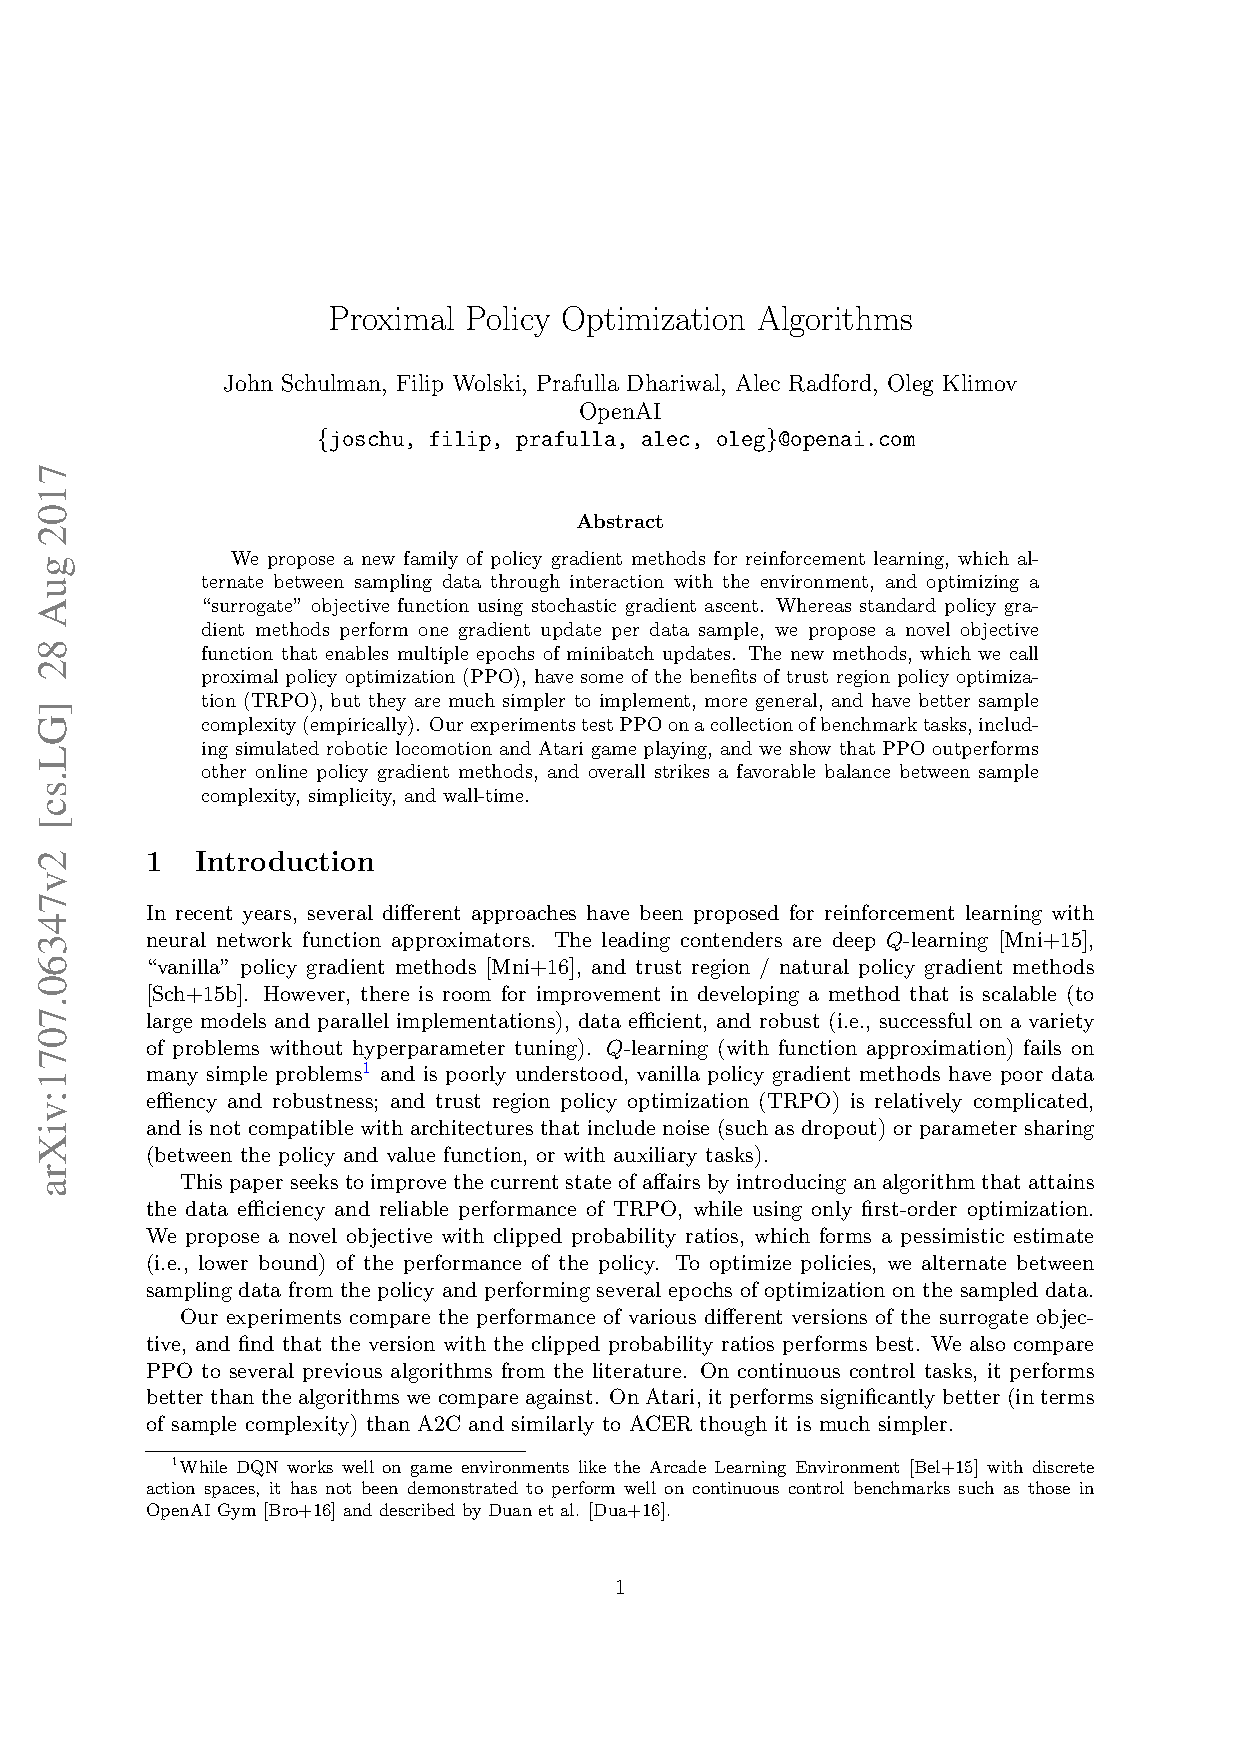
\includepdf[pages=-,pagecommand={\thispagestyle{empty}}]{pdfs/schulman-2017-ppo.pdf}

\papertoclabel{[2017] Deep Reinforcement Learning from Human Preferences (Christiano et al.)}{paper:christiano-2017-rlhf}{\index{Christiano, Paul}\index{Leike, Jan}\index{Brown, Tom}\index{Martic, Miljan}\index{Legg, Shane}\index{Amodei, Dario}}
\input{content/summary-christiano-2017-rlhf}
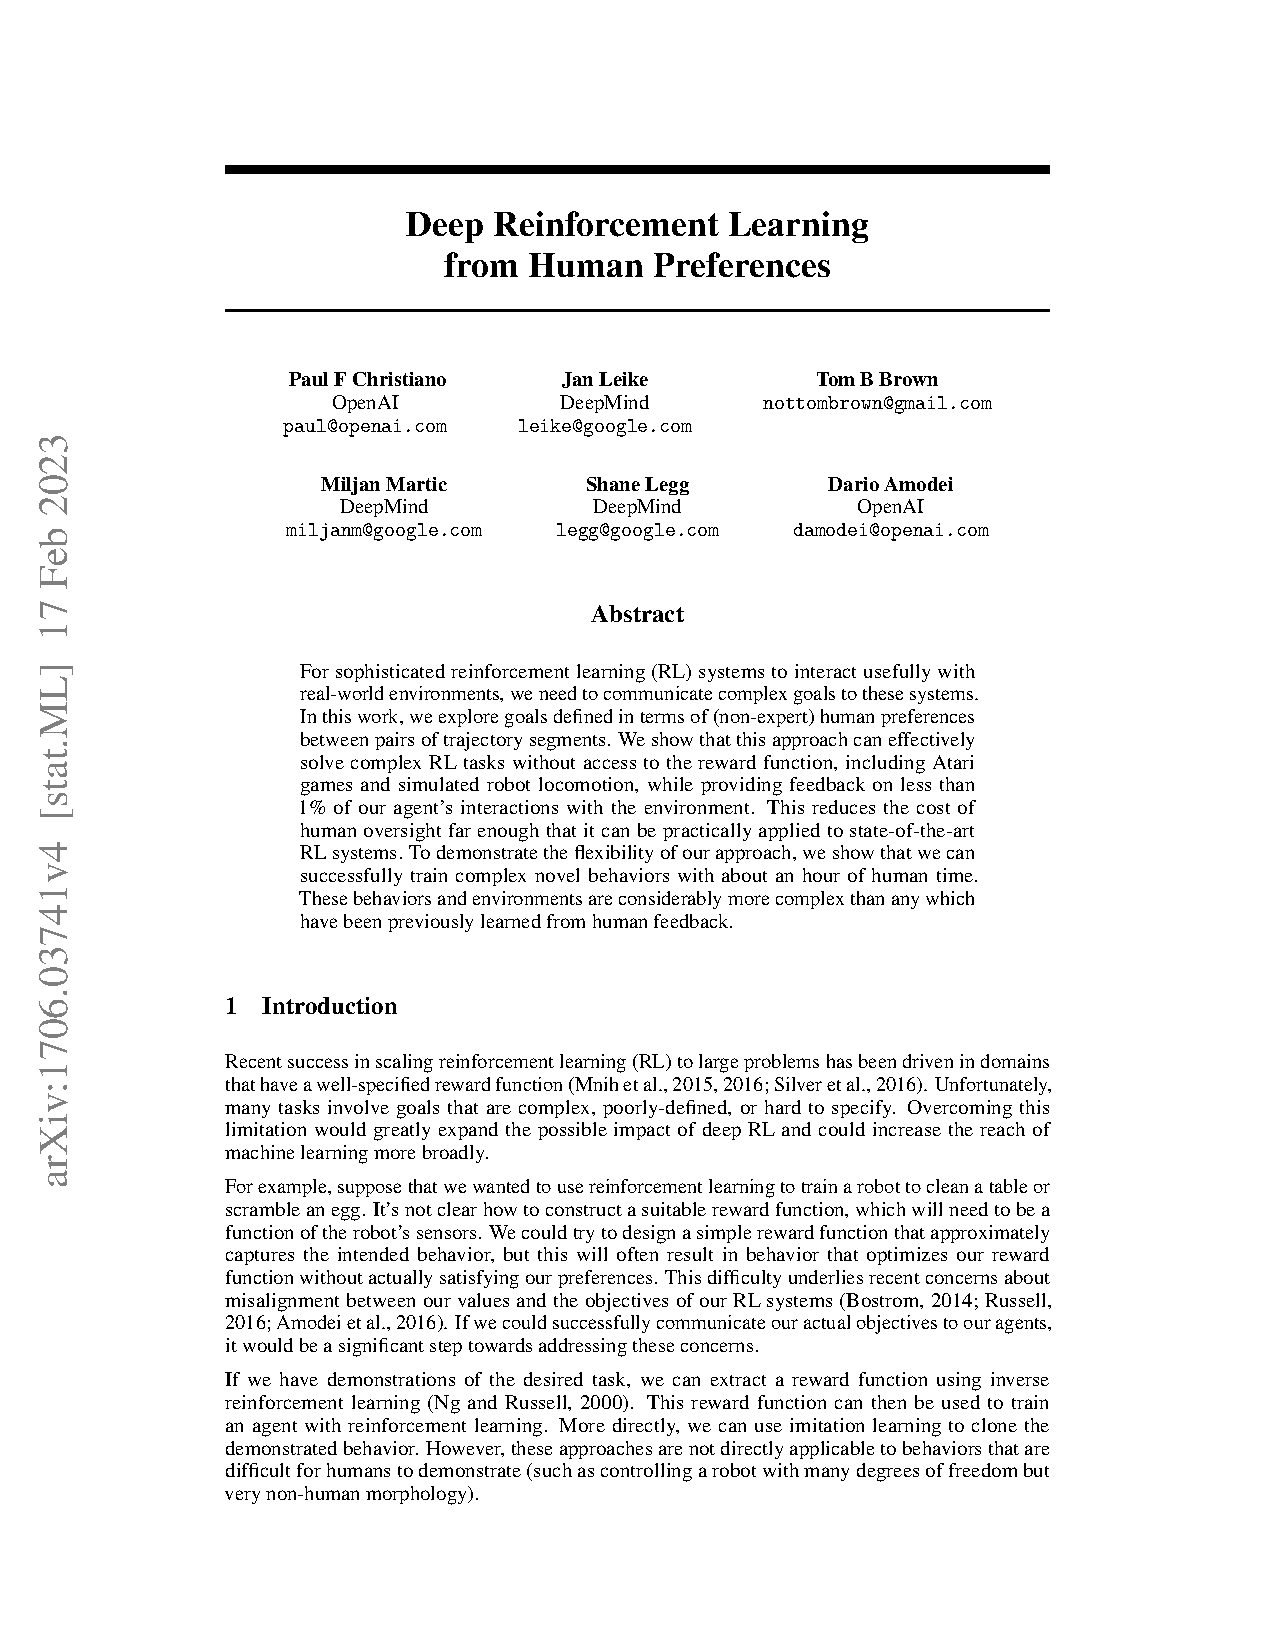
\includepdf[pages=-,pagecommand={\thispagestyle{empty}}]{pdfs/christiano-2017-rlhf.pdf}

\papertoclabel{[2017] Decoupled Weight Decay Regularization (Loshchilov \& Hutter)}{paper:loshchilov-2017-adamw}{\index{Loshchilov, Ilya}\index{Hutter, Frank}}
% Paper Summary: Decoupled Weight Decay Regularization (Loshchilov & Hutter, 2017)

\begin{papersummary}{2017}{Decoupled Weight Decay Regularization}{Ilya Loshchilov, Frank Hutter}{AdamW corrects the interaction between adaptive gradient methods and weight decay by decoupling the decay term from the gradient update, producing the optimizer used to pretrain nearly every large language model.}

\summaryheading{Key Ideas}
For plain stochastic gradient descent, L2 regularization and weight decay are equivalent; the paper shows that for adaptive methods such as Adam (\hyperref[paper:kingma-ba-2014]{Kingma \& Ba, 2014}) they are not. When the L2 penalty flows through Adam's adaptive rescaling, weights with large historical gradients are regularized less than intended, which partly explained Adam's reputation for generalizing worse than tuned SGD. The proposed fix decouples the decay: weights are shrunk directly at each step, outside the gradient-based update. The resulting optimizer, AdamW, restores the intended regularization, decouples the optimal decay factor from the learning rate, and simplifies hyperparameter search. The paper also pairs the decoupled update with the cosine warm-restart schedule the same authors had introduced in SGDR, yielding the AdamWR variant.

\summaryheading{Follow-on Works}
AdamW displaced Adam as the default for training transformers: BERT, GPT-3, and essentially every subsequent large language model pretrains with AdamW under a warmup-then-decay schedule. Its per-parameter second-moment state, stored in addition to momentum, set the memory budget that drove follow-on work on sharded optimizer states and low-precision optimizer variants. Not until the Muon optimizer (\hyperref[paper:liu-2025-muon]{Liu et al., 2025}) did a successor demonstrate a material compute-efficiency advantage over AdamW at frontier scale.

\summaryheading{Lasting Contributions}
The decoupled update is now what practitioners mean by ``weight decay'' in deep learning. A decade of frontier models, across dense and mixture-of-experts architectures, has been trained with the algorithm essentially as published. The result came from noticing that two formulations treated as equivalent were not, and showing that the difference mattered at practical scale.

\end{papersummary}

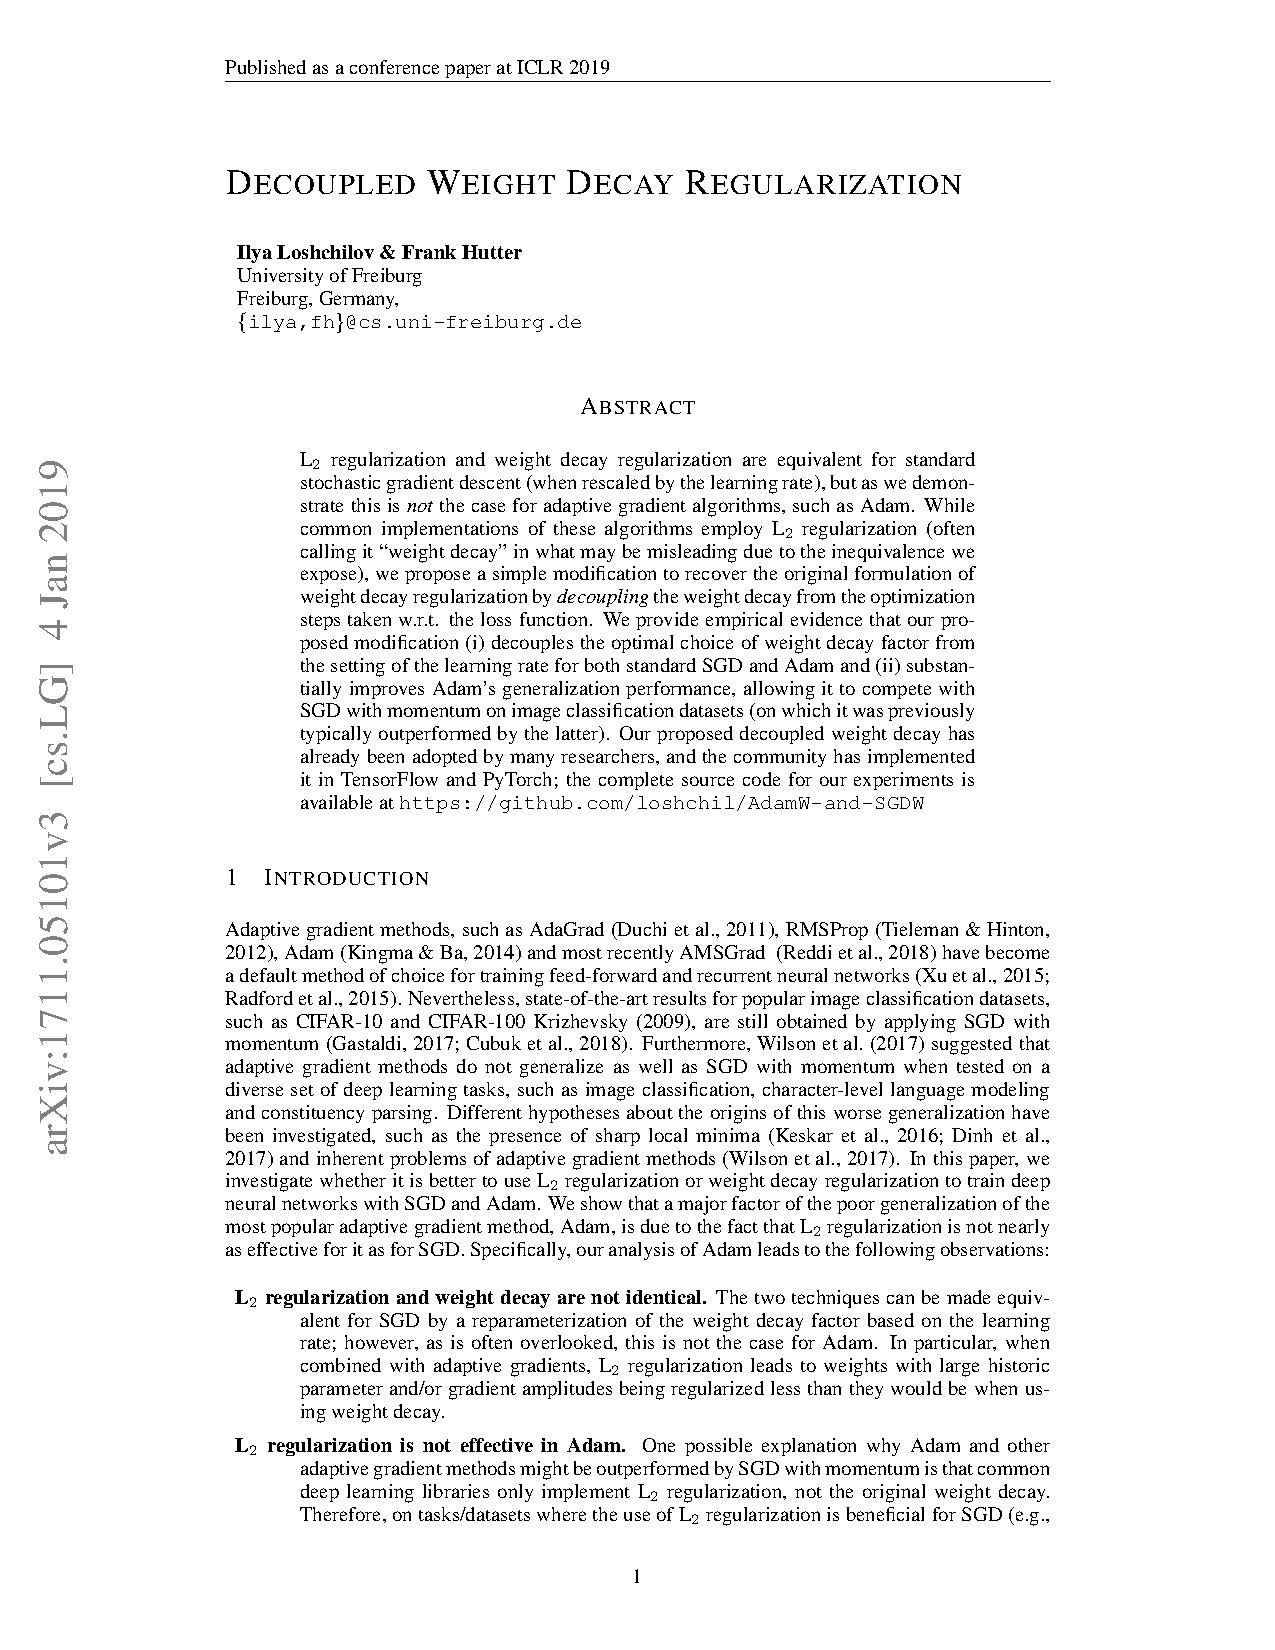
\includepdf[pages=-,pagecommand={\thispagestyle{empty}}]{pdfs/loshchilov-2017-adamw.pdf}

\papertoclabel{[2018] Deep Contextualized Word Representations (Peters et al.)}{paper:peters-2018}{\index{Peters, Matthew E.}\index{Neumann, Mark}\index{Iyyer, Mohit}\index{Gardner, Matt}\index{Clark, Christopher}\index{Lee, Kenton}\index{Zettlemoyer, Luke}}
\input{content/summary-peters-2018}
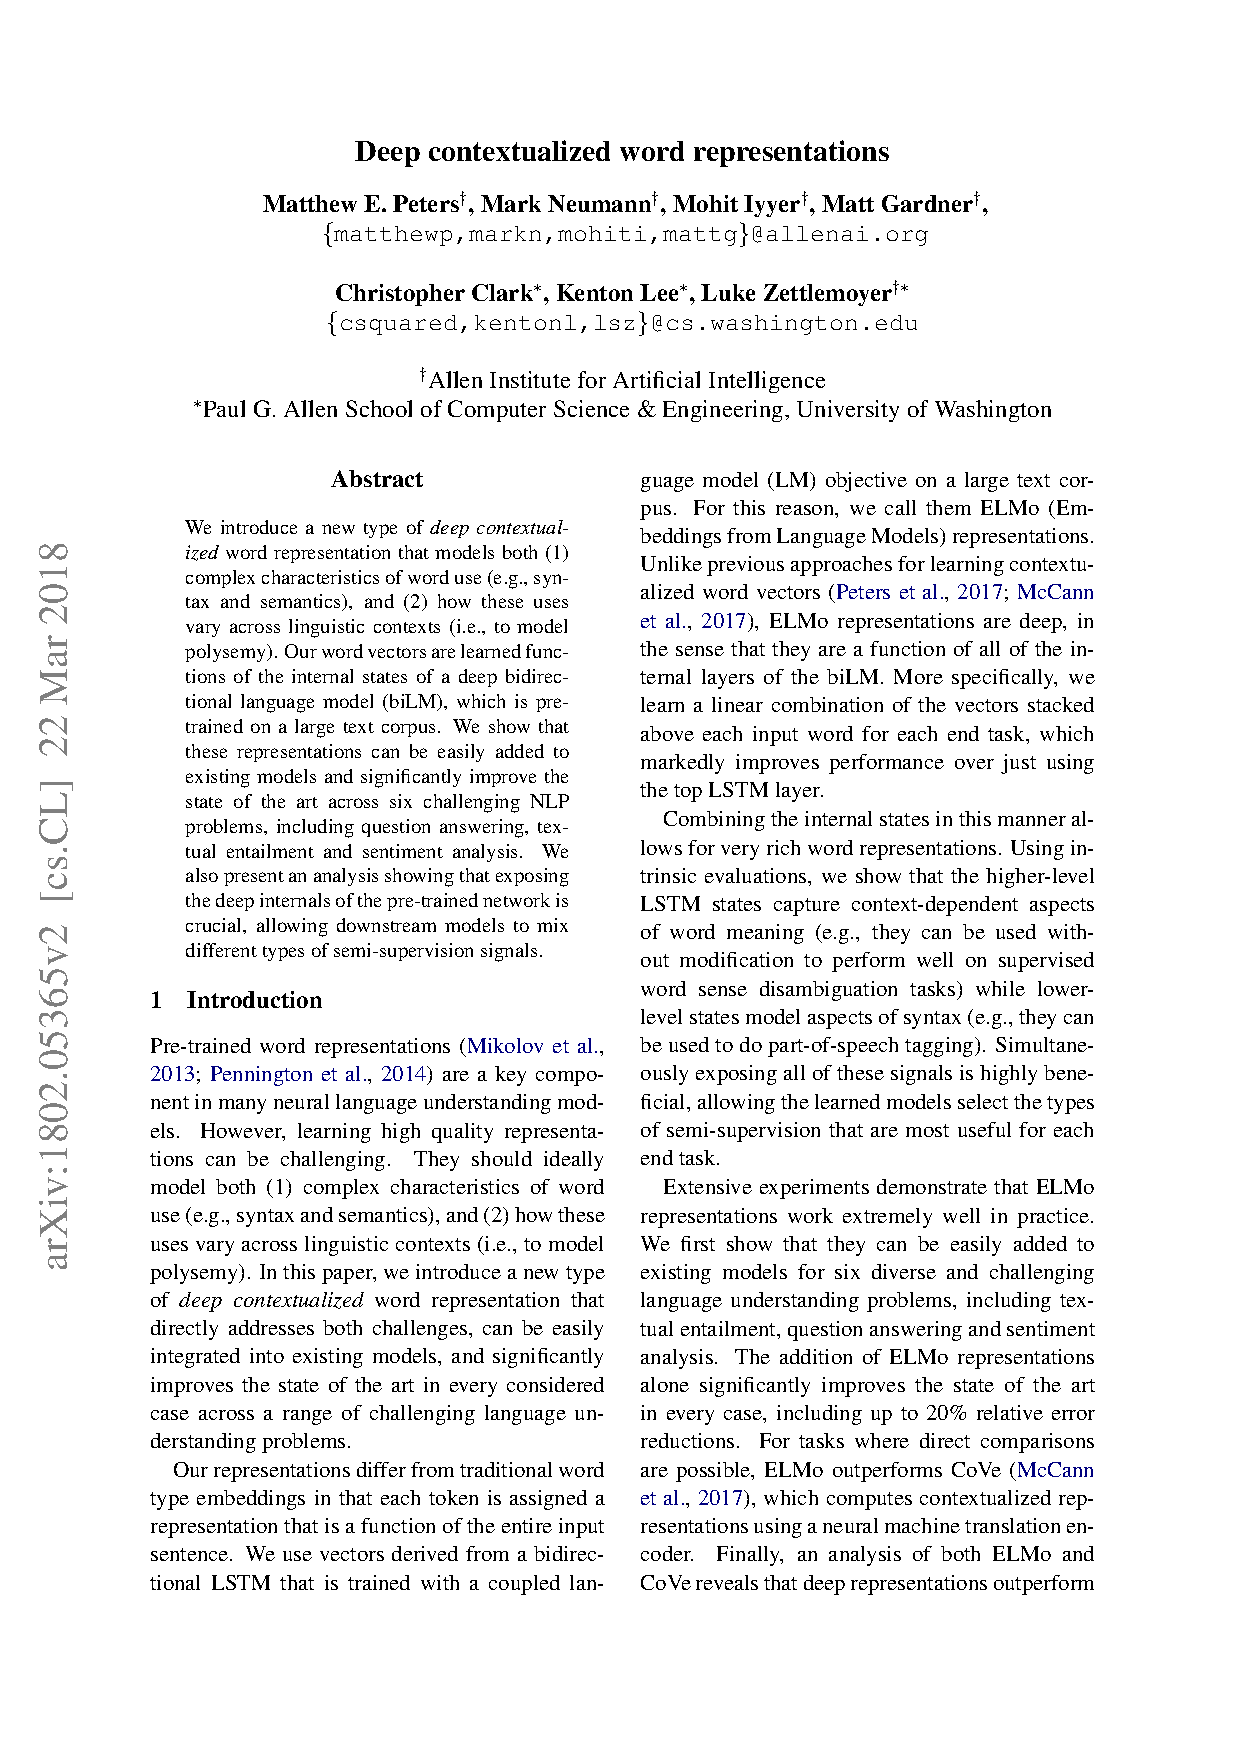
\includepdf[pages=-,pagecommand={\thispagestyle{empty}}]{pdfs/peters-2018.pdf}

\papertoclabel{[2018] BERT: Pre-training of Deep Bidirectional Transformers (Devlin et al.)}{paper:devlin-2018}{\index{Devlin, Jacob}\index{Chang, Ming-Wei}\index{Lee, Kenton}\index{Toutanova, Kristina}}
\input{content/summary-devlin-2018}
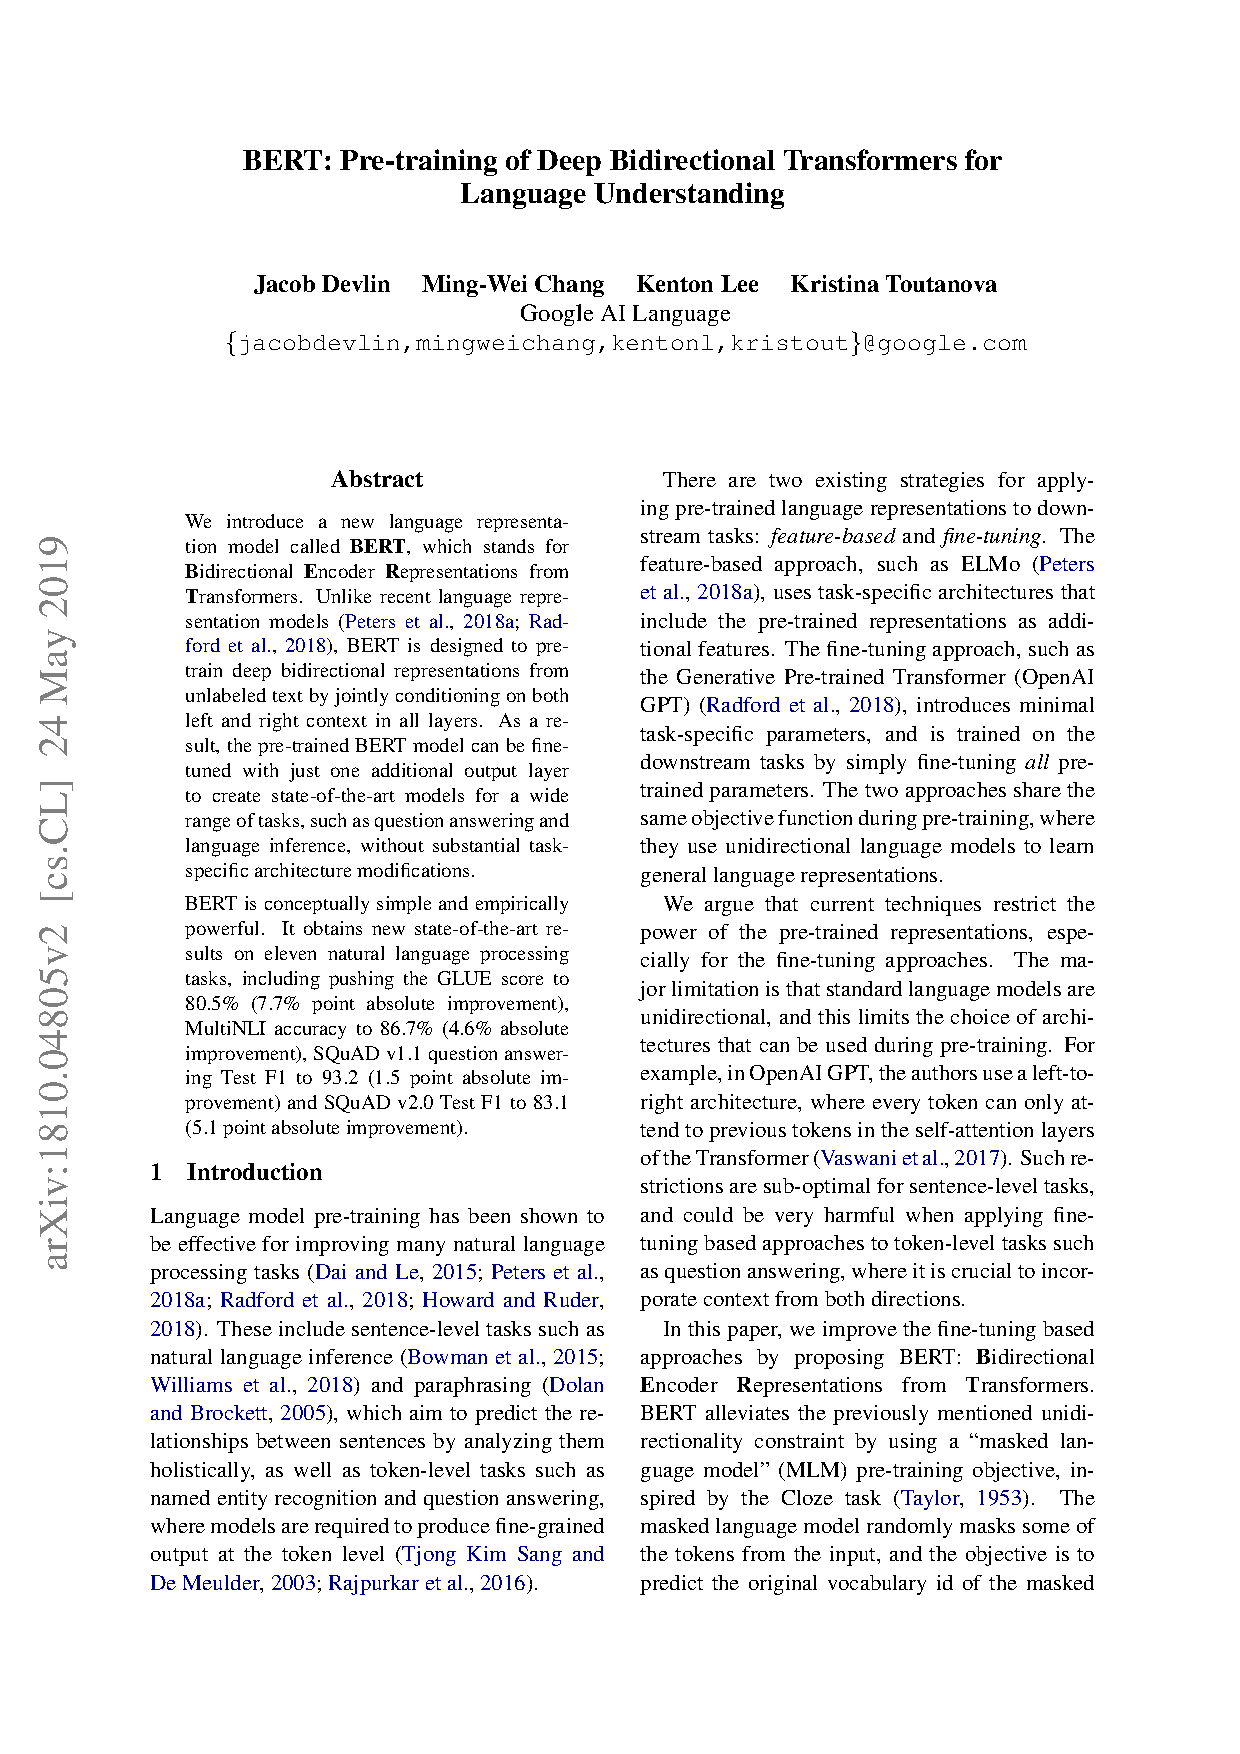
\includepdf[pages=-,pagecommand={\thispagestyle{empty}}]{pdfs/devlin-2018.pdf}

\papertoclabel{[2018] Improving Language Understanding by Generative Pre-Training (Radford et al.)}{paper:radford-2018}{\index{Radford, Alec}\index{Narasimhan, Karthik}\index{Salimans, Tim}\index{Sutskever, Ilya}}
\input{content/summary-radford-2018}
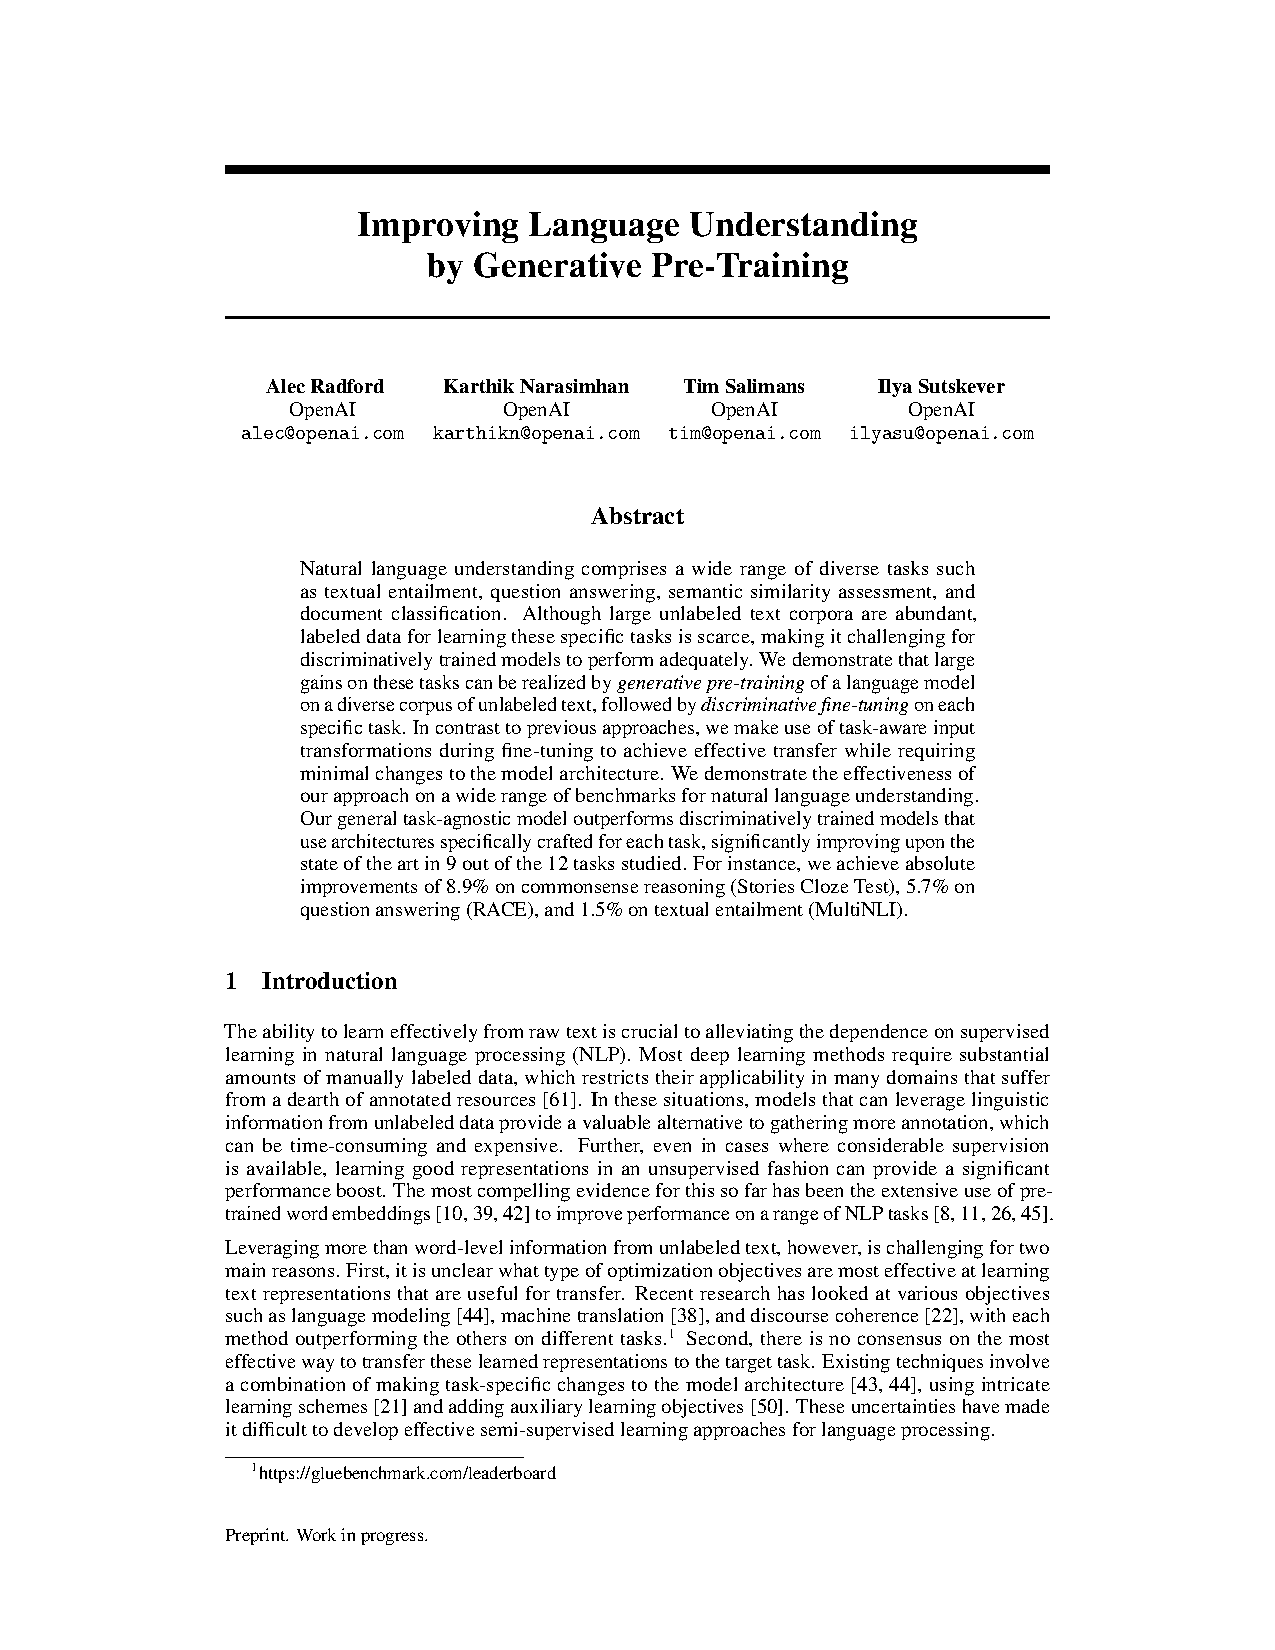
\includepdf[pages=-,pagecommand={\thispagestyle{empty}}]{pdfs/radford-2018.pdf}

\papertoclabel{[2019] Exploring the Limits of Transfer Learning with a Unified Text-to-Text Transformer (Raffel et al.)}{paper:raffel-2019}{\index{Raffel, Colin}\index{Shazeer, Noam}\index{Roberts, Adam}\index{Lee, Katherine}\index{Narang, Sharan}\index{Matena, Michael}\index{Zhou, Yanqi}\index{Li, Wei}\index{Liu, Peter J.}}
\input{content/summary-raffel-2019}
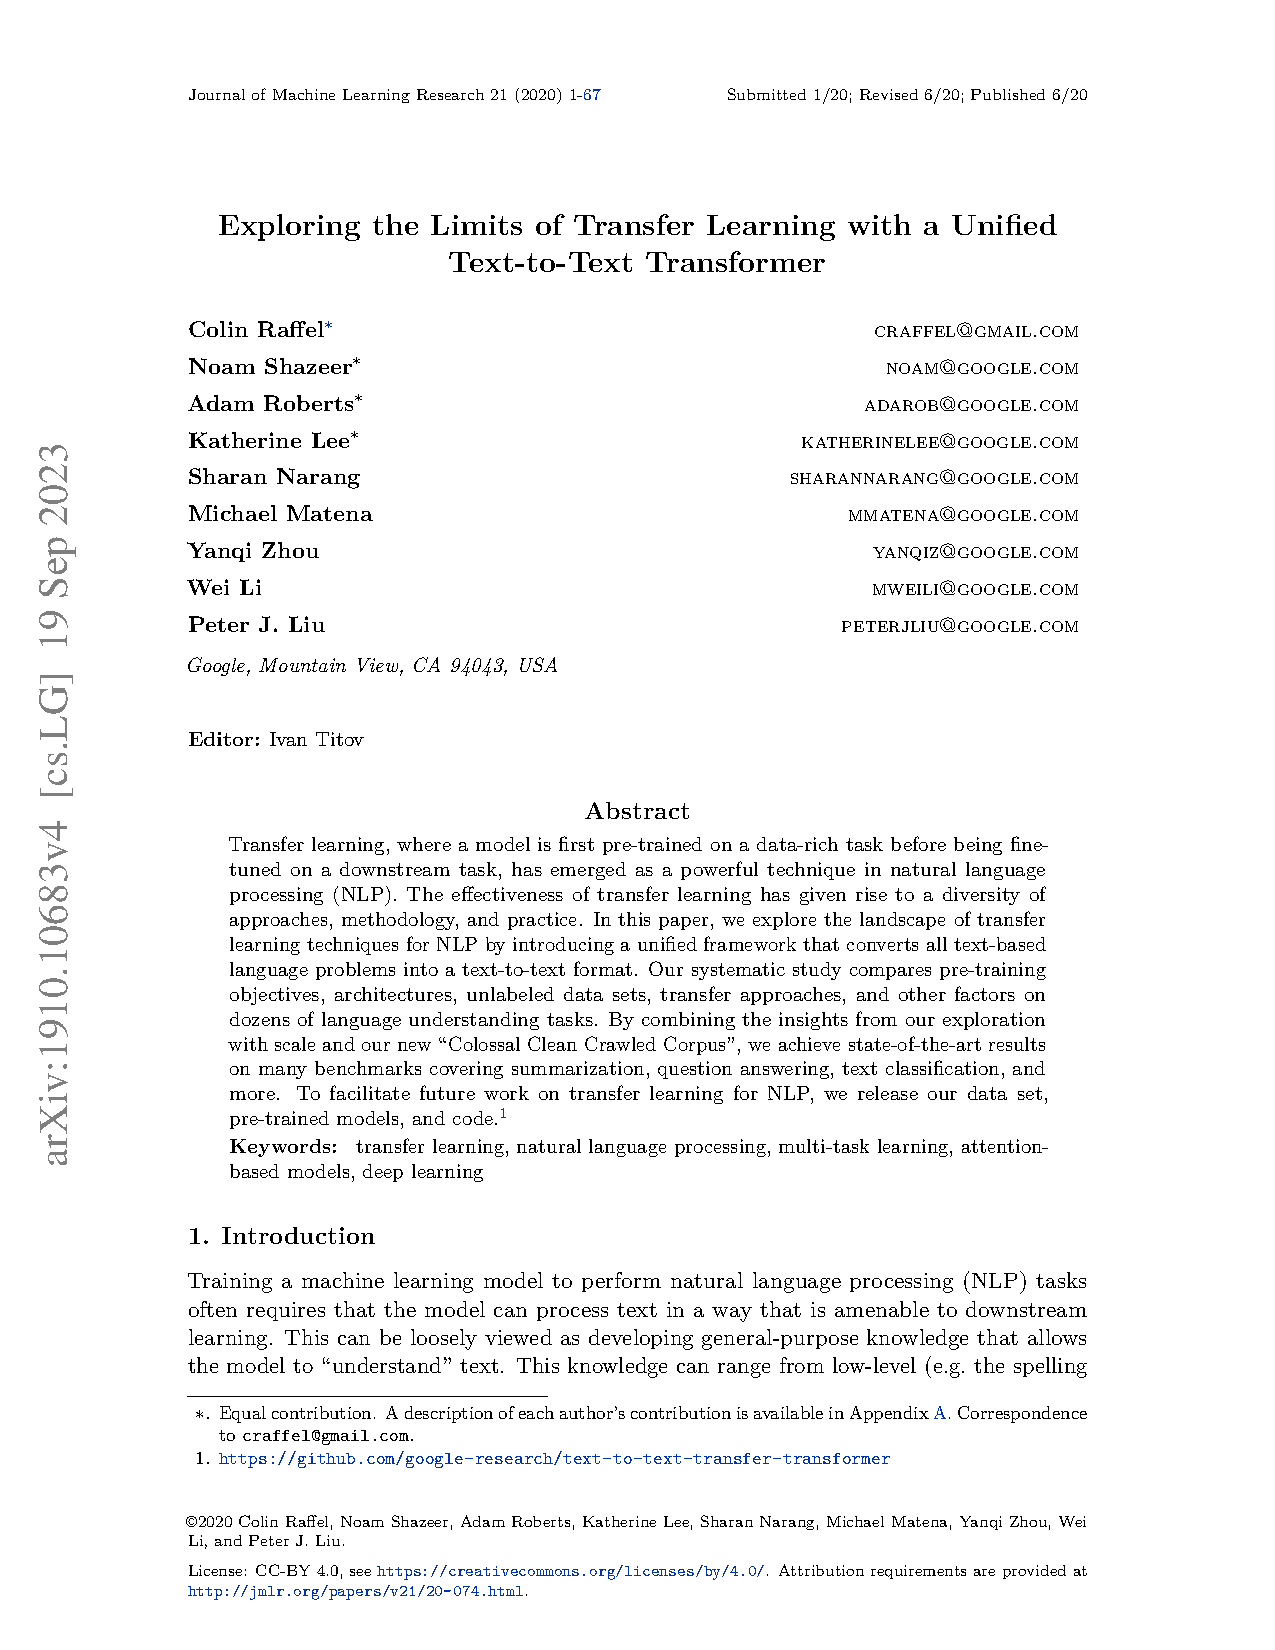
\includepdf[pages=-,pagecommand={\thispagestyle{empty}}]{pdfs/raffel-2019.pdf}



% Part V: Emergence and Scale (2019–2020)
\part[Emergence and Scale]{Emergence and Scale\texorpdfstring{\\}{, }2019--2020}
\input{content/part5-chapter-new}

% Part VI: Efficiency, Alignment, and Reasoning (2021–2022)
\part[Efficiency, Alignment, and Reasoning]{Efficiency, Alignment, and Reasoning\texorpdfstring{\\}{, }2021--2022}
\input{content/part6-chapter-new}

% Part VII: Open LLMs and Modern Frontier (2023–2024)
\part[Open LLMs and Modern Frontier]{Open LLMs and Modern Frontier\texorpdfstring{\\}{, }2023--2024}
\input{content/part7-chapter-new}

% Part VIII: Reasoning and the Open Frontier (2024–2026)
\part[Reasoning and the Open Frontier]{Reasoning and the Open Frontier\texorpdfstring{\\}{, }2024--2026}
% Part VIII: Reasoning and the Open Frontier (2024-2026)

\PartIntroChapter{Introduction to Part VIII}

The period from 2024 to 2026 was defined by two developments. First, reinforcement learning moved from the periphery of the training pipeline to its center: models learned to reason---to produce long chains of intermediate computation, verify their own work, and backtrack---by optimizing against rewards that could be checked mechanically. Second, open models closed the gap with proprietary frontier systems, and in doing so documented publicly the full stack of techniques that frontier training requires.

The algorithmic substrate for the reasoning shift was laid by Shao and colleagues, whose Group Relative Policy Optimization (GRPO) removed the learned value network from PPO\index{GRPO (Group Relative Policy Optimization)} and estimated advantages from groups of sampled responses to the same prompt, removing a second model of comparable size from the training loop and simplifying its tuning. Lambert and colleagues introduced reinforcement learning with verifiable rewards (RLVR)\index{verifiable rewards (RLVR)}, replacing the learned reward model with programmatic checks---exact-match answers in mathematics, constraint satisfaction in instruction following---and released the complete T\"ulu~3 recipe, data, and code. Both ideas are visible, arrived at independently, in DeepSeek-R1. Its central experiment, R1-Zero, applied reinforcement learning with rule-based rewards directly to a base model, with no supervised reasoning traces, and produced emergent self-verification and reflection; the full R1 pipeline added a small cold-start corpus and a second RL stage, matching OpenAI's o1 and validating at production scale the test-time-compute findings that closed Part~VII. R1 further showed that reasoning behavior elicited by RL in a large model transfers to small models through simple distillation.

Architecture continued to move beyond the dense transformer. Gloeckle and colleagues showed that predicting several future tokens through parallel heads\index{multi-token prediction} improves sample efficiency and provides native draft heads for speculative decoding. Wang and colleagues removed the auxiliary balancing losses from mixture-of-experts routing\index{auxiliary-loss-free load balancing}, steering expert load through a feedback-controlled bias rather than an objective that competes with the language-modeling gradient. The Kimi team's Kimi Delta Attention---a fine-grained gated delta rule\index{Kimi Delta Attention} interleaved with periodic full-attention layers---became the first hybrid linear-attention architecture to outperform full attention under controlled comparisons, making million-token contexts economical. Elango and colleagues restructured the expert layer itself, routing compressed latent representations\index{LatentMoE} to experts to maximize accuracy per unit of compute and memory. On the training side, Liu and colleagues demonstrated that Muon, a matrix-orthogonalizing optimizer, scales to large-model pretraining\index{Muon optimizer} with roughly twice the computational efficiency of AdamW---the first credible successor to AdamW in the optimizer lineage that runs through this collection from Adam onward.

These techniques are the components from which the era's production systems were assembled. DeepSeek-V3 combined multi-head latent attention, auxiliary-loss-free routing, and multi-token prediction at 671 billion parameters; Llama~3, Gemma~3, and Qwen3 documented open recipes for dense frontier training, quantized deployment, and controllable reasoning effort; and Kimi K2 carried a stabilized Muon variant to trillion-parameter pretraining, with K3 adding delta attention and latent expert routing at million-token context. The papers collected below are the foundational methods those systems build on.

\section*{Papers in This Section}

\begin{enumerate}
\item \textbf{Shao et al. (2024)} --- DeepSeekMath introduces GRPO: critic-free policy optimization with group-relative advantages, the standard algorithm of the reasoning era.

\item \textbf{Gloeckle et al. (2024)} --- Multi-token prediction: parallel next-$n$-token heads improving sample efficiency and enabling self-speculative decoding.

\item \textbf{Wang et al. (2024)} --- Auxiliary-loss-free load balancing: feedback-controlled routing bias replacing balancing losses in mixture-of-experts training.

\item \textbf{Lambert et al. (2024)} --- T\"ulu~3: reinforcement learning with verifiable rewards and a fully open post-training recipe.

\item \textbf{DeepSeek-AI (2025)} --- DeepSeek-R1: pure reinforcement learning elicits emergent reasoning without supervised traces, distillable to small models.

\item \textbf{Liu et al. (2025)} --- Muon at scale: matrix orthogonalization roughly doubling pretraining compute efficiency over AdamW.

\item \textbf{Kimi Team (2025)} --- Kimi Linear: fine-grained gated delta attention in hybrid layers, outperforming full attention at a fraction of its memory cost.

\item \textbf{Elango et al. (2026)} --- LatentMoE: expert computation in a compressed latent space, maximizing accuracy per FLOP and per parameter.
\end{enumerate}


% Papers follow
% Part VIII Papers: Reasoning and the Open Frontier (2024–2026)

\addcontentsline{toc}{subsection}{[2024] DeepSeekMath: Pushing the Limits of Mathematical Reasoning in Open Language Models (Shao et al.)}
\phantomsection
\label{paper:shao-2024-grpo}
% Paper Summary: DeepSeekMath: Pushing the Limits of Mathematical Reasoning in Open Language Models (Shao et al., 2024)

\begin{papersummary}{2024}{DeepSeekMath: Pushing the Limits of Mathematical Reasoning in Open Language Models}{Zhihong Shao, Peiyi Wang, Qihao Zhu, Runxin Xu, Junxiao Song, et al. (DeepSeek-AI)}{DeepSeekMath introduced Group Relative Policy Optimization (GRPO), a critic-free simplification of PPO whose group-relative advantage estimates became the standard reinforcement learning algorithm of the reasoning era.}

\summaryheading{Key Ideas}
The paper makes two contributions. The first is a data pipeline that extracts 120B tokens of mathematical text from Common Crawl through iterative classifier bootstrapping, showing that web-scale corpora contain far more high-quality domain data than curated collections had suggested; the resulting 7B model approaches the mathematical reasoning of far larger closed models. The second is Group Relative Policy Optimization. PPO (\hyperref[paper:schulman-2017-ppo]{Schulman et al., 2017}) requires a learned value network, typically as large as the policy, to estimate advantages. GRPO eliminates it: for each prompt, the policy samples a group of responses, and each response's advantage is its reward standardized against the group mean and variance. This removes a second model of comparable size from the training loop, eliminates the critic's instabilities, and aligns naturally with outcome-based rewards, where credit assignment over a whole response is precisely what a group baseline provides.

\summaryheading{Follow-on Works}
GRPO became the default optimizer of reasoning-focused reinforcement learning. DeepSeek-R1 (\hyperref[paper:deepseek-2025-r1]{DeepSeek-AI, 2025}) used it to elicit emergent chain-of-thought reasoning from a base model with purely rule-based rewards, and open post-training recipes converged on it alongside the verifiable-rewards paradigm of T\"ulu~3 (\hyperref[paper:lambert-2024-tulu3]{Lambert et al., 2024}). A family of refinements---DAPO, Dr.~GRPO, and GSPO among them---adjusted its clipping, normalization, and length handling for long reasoning traces, while frontier systems from Qwen3 to Kimi K2 and K3 applied GRPO-descended objectives across reasoning, agentic, and coding domains.

\summaryheading{Lasting Contributions}
GRPO reduced reinforcement learning on language models to sampling a group of responses, standardizing their rewards, and ascending the policy gradient under a KL constraint. That simplicity made large-scale RL accessible to the open community and turned post-training RL from a fragile final step into a primary axis of capability scaling. The 7B model's performance in a formal domain also showed that targeted data and targeted optimization can substitute for parameter count.

\end{papersummary}

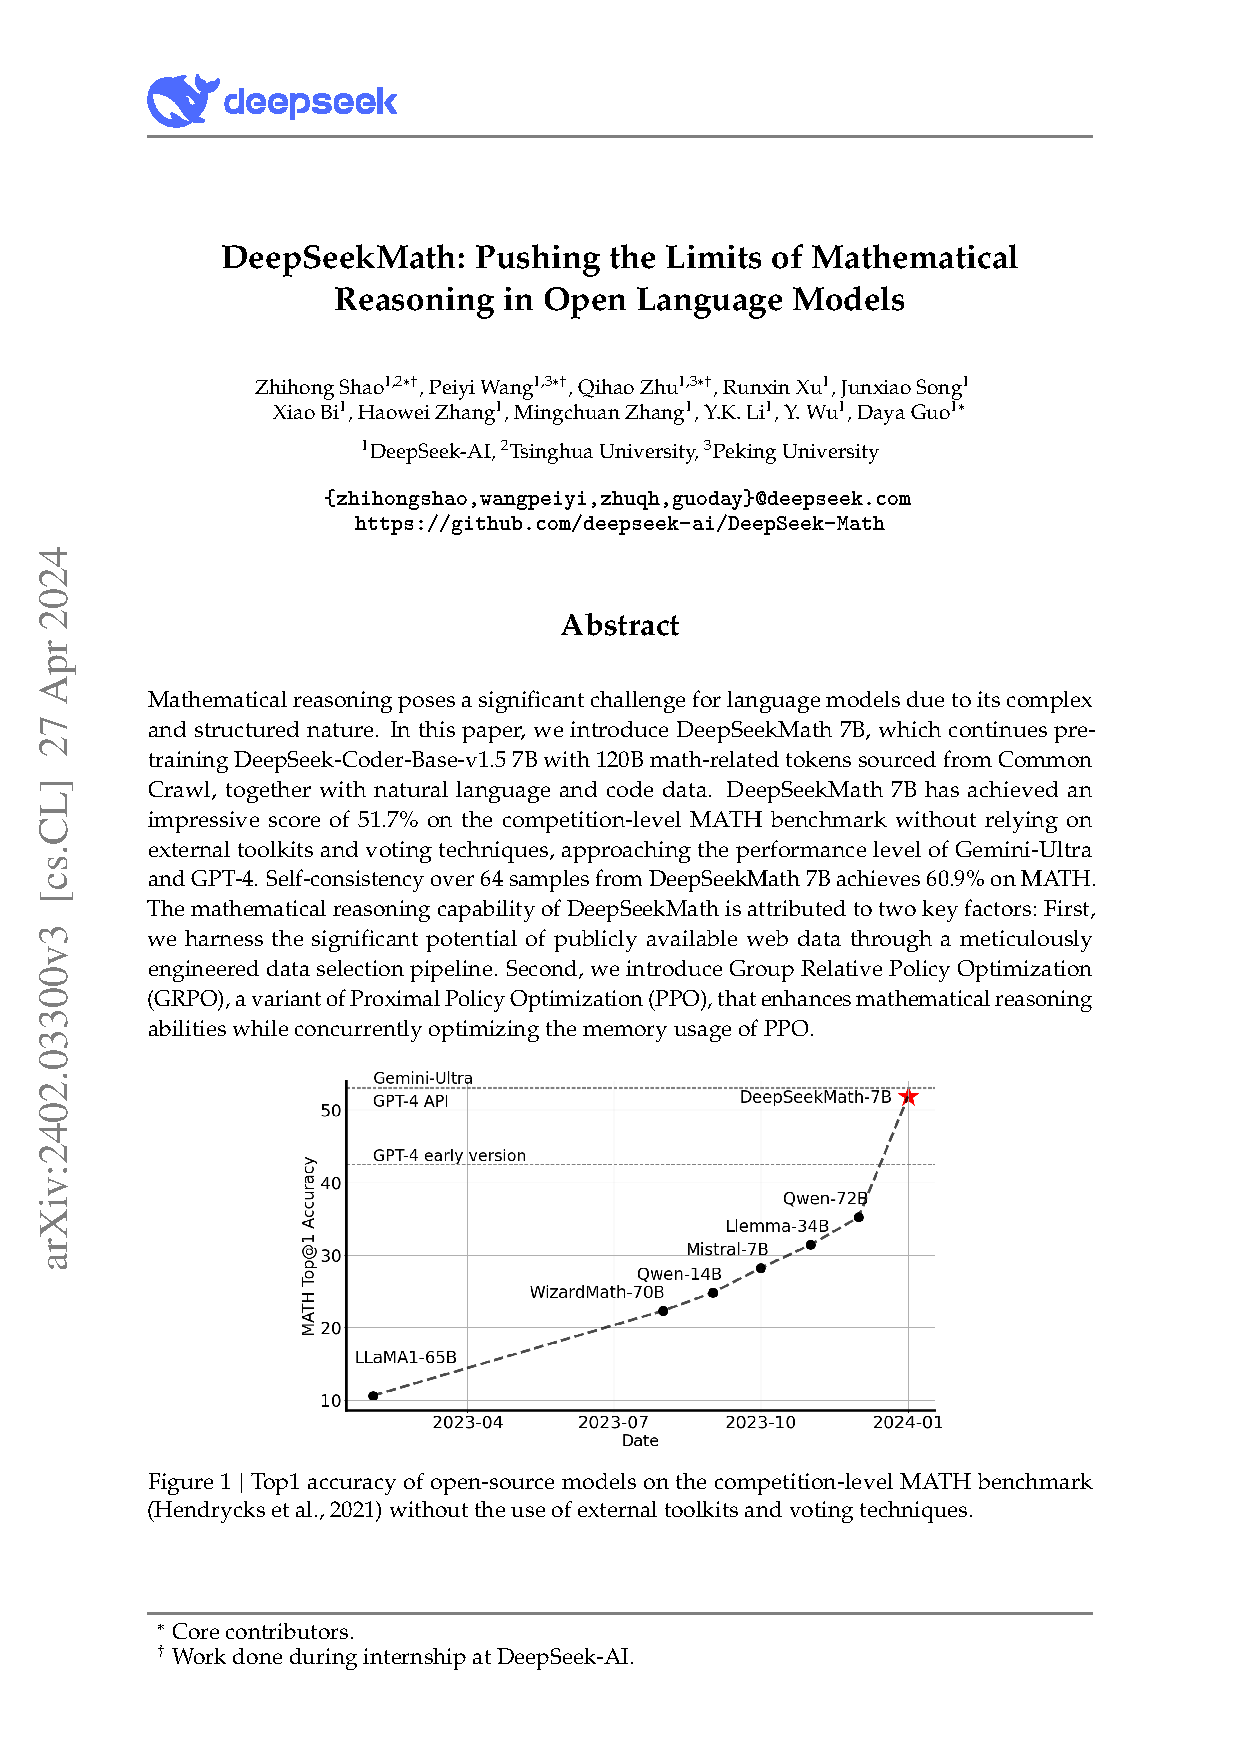
\includepdf[pages=-,pagecommand={}]{pdfs/shao-2024-grpo.pdf}

\addcontentsline{toc}{subsection}{[2024] Better \& Faster Large Language Models via Multi-token Prediction (Gloeckle et al.)}
\phantomsection
\label{paper:gloeckle-2024-mtp}
% Paper Summary: Better & Faster Large Language Models via Multi-token Prediction (Gloeckle et al., 2024)

\begin{papersummary}{2024}{Better \& Faster Large Language Models via Multi-token Prediction}{Fabian Gloeckle, Badr Youbi Idrissi, Baptiste Rozi\`ere, David Lopez-Paz, Gabriel Synnaeve}{Training language models to predict several future tokens through parallel output heads improves sample efficiency, particularly on code, and equips models with native draft heads for self-speculative decoding.}

\summaryheading{Key Ideas}
Next-token prediction, the objective underlying the GPT line (\hyperref[paper:radford-2019]{Radford et al., 2019}), teaches a model to be locally correct while remaining shortsighted about the structure of what follows. The paper attaches $n$ output heads to a shared trunk, each predicting one of the next $n$ tokens, and trains them jointly with negligible overhead by computing head gradients sequentially rather than materializing all logits at once. The auxiliary predictions act as a lookahead regularizer: representations must encode not just the next token but the local future, which measurably shifts capability on generative benchmarks---13B-parameter models solve 12\% more HumanEval problems and 17\% more MBPP problems than next-token baselines---with benefits that grow with model size and persist through fine-tuning. At inference, the extra heads draft future tokens that the primary head verifies, yielding up to threefold self-speculative decoding speedups (\hyperref[paper:leviathan-2022-speculative]{Leviathan et al., 2022}) without an external draft model.

\summaryheading{Follow-on Works}
DeepSeek-V3 adopted a sequential variant of multi-token prediction as both auxiliary training objective and speculative draft head at 671B-parameter scale, crediting it with measurable quality gains, and subsequent frontier mixture-of-experts models including the Kimi K series retained MTP modules for the same dual purpose. The technique also informed research on lookahead objectives and register tokens as means of giving autoregressive models explicit representations of their own future output.

\summaryheading{Lasting Contributions}
The paper converted a long-standing intuition---that pure next-token prediction underuses the training signal---into a deployable objective with no inference-time cost and a built-in acceleration mechanism. Multi-token prediction is now a standard component of frontier pretraining recipes.

\end{papersummary}

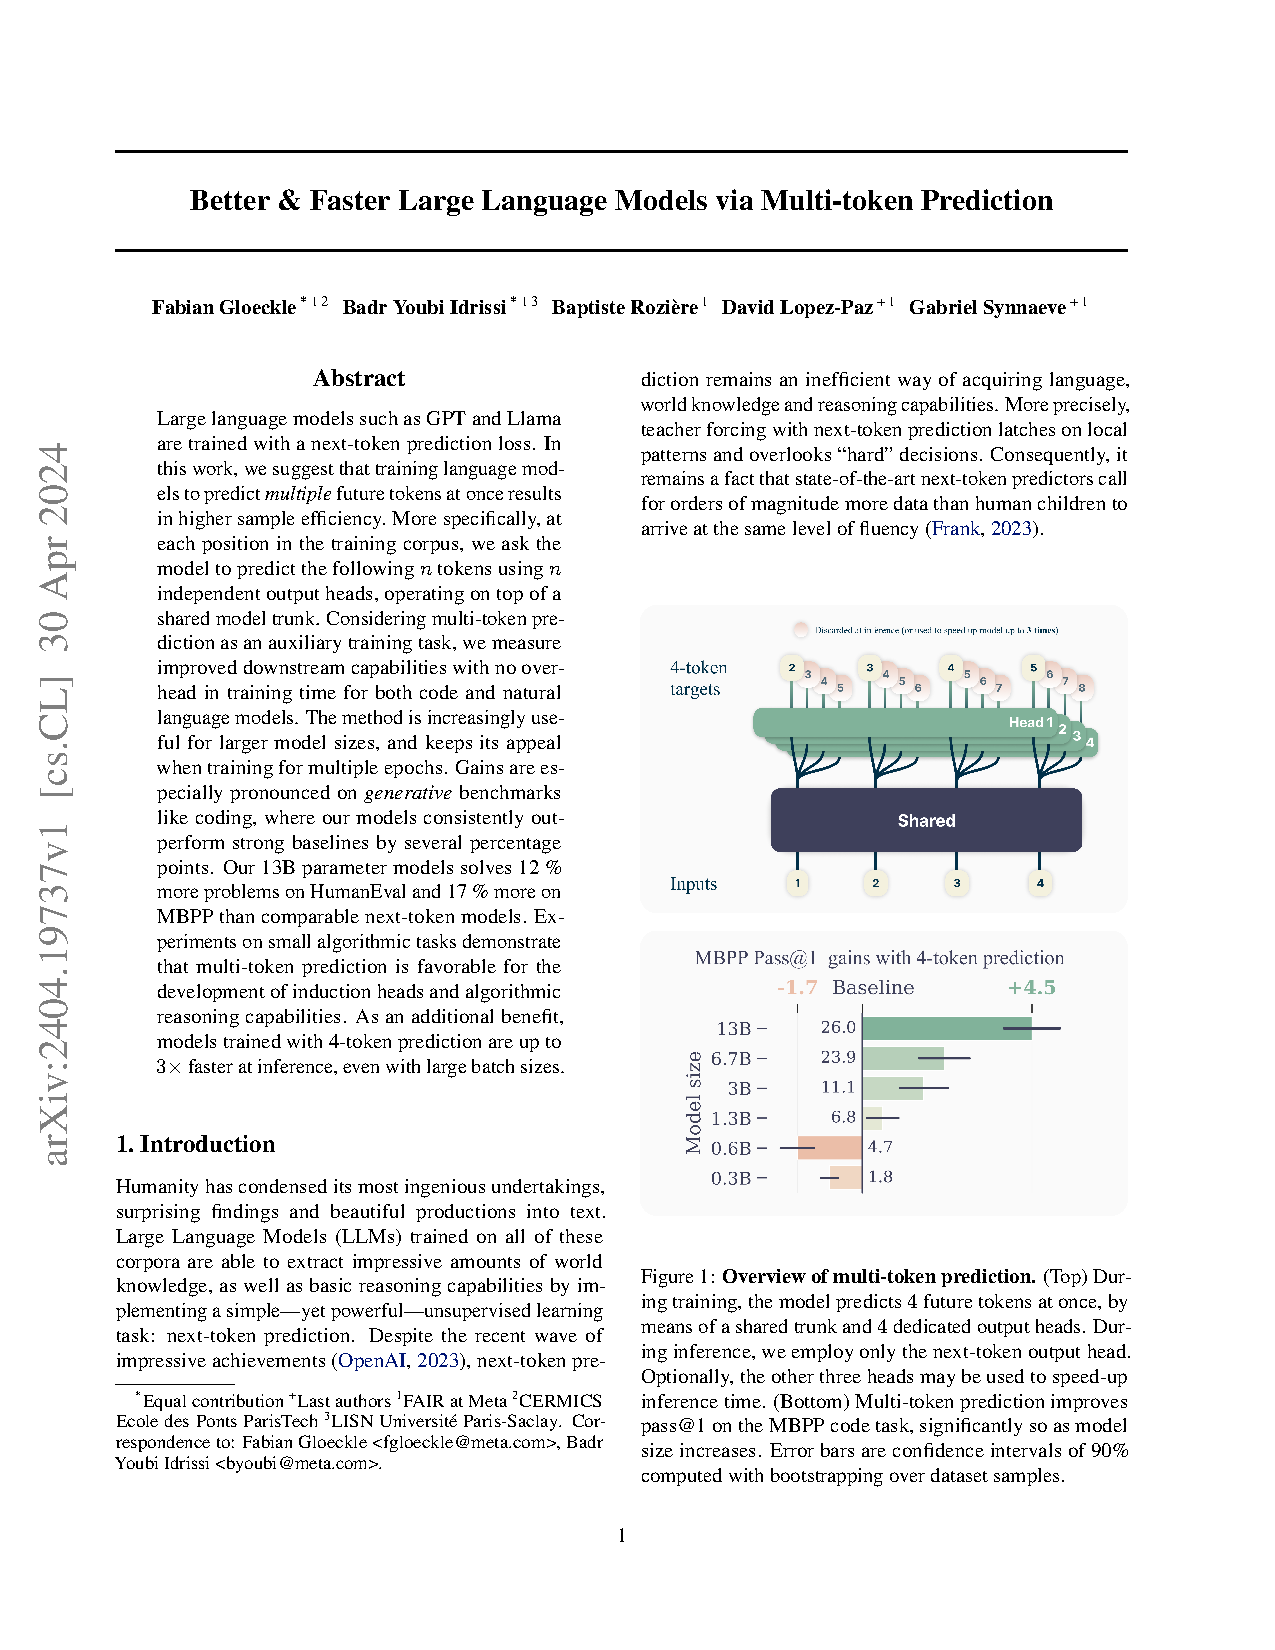
\includepdf[pages=-,pagecommand={}]{pdfs/gloeckle-2024-mtp.pdf}

\addcontentsline{toc}{subsection}{[2024] Auxiliary-Loss-Free Load Balancing Strategy for Mixture-of-Experts (Wang et al.)}
\phantomsection
\label{paper:wang-2024-auxfree}
% Paper Summary: Auxiliary-Loss-Free Load Balancing Strategy for Mixture-of-Experts (Wang et al., 2024)

\begin{papersummary}{2024}{Auxiliary-Loss-Free Load Balancing Strategy for Mixture-of-Experts}{Lean Wang, Huazuo Gao, Chenggang Zhao, Xu Sun, Damai Dai}{Loss-free balancing steers mixture-of-experts routing with a feedback-controlled per-expert bias instead of an auxiliary loss, removing the gradient interference that balancing objectives impose on the language-modeling task.}

\summaryheading{Key Ideas}
Sparse mixture-of-experts layers collapse unless token load is spread across experts, and since Shazeer's original formulation (\hyperref[paper:shazeer-2017-moe]{Shazeer et al., 2017}) the standard remedy had been an auxiliary balancing loss whose gradients tug against the language-modeling objective: weight it strongly and quality suffers, weakly and routing collapses. The paper removes the loss entirely. Each expert carries a bias added to its routing score only for top-$k$ selection---the bias never touches the gating weights that mix expert outputs---and a simple feedback rule adjusts it between steps, raising the bias of underloaded experts and lowering that of overloaded ones. Balance becomes a control problem rather than an optimization term, leaving the training gradient entirely dedicated to the task. Experiments show simultaneously better perplexity and better load balance than auxiliary-loss training, with none of the batch-composition pathologies of alternatives such as expert choice routing.

\summaryheading{Follow-on Works}
DeepSeek-V3 adopted the strategy as its principal balancing mechanism at 671B parameters, demonstrating stable training of 256-expert layers with only a vestigial sequence-level loss as a safeguard, and it became the reference approach for subsequent large sparse models. Refinements such as the quantile-based balancing used in Kimi K3's latent mixture-of-experts extend the same feedback principle, and the design recurs in the fine-grained expert regimes explored by LatentMoE (\hyperref[paper:elango-2026-latentmoe]{Elango et al., 2026}) and analyzed in the scaling laws of \hyperref[paper:krajewski-2024]{Krajewski et al.\ (2024)}.

\summaryheading{Lasting Contributions}
The paper resolved a tension that had constrained mixture-of-experts training since its modern inception: the mechanism that keeps experts alive no longer competes with the objective that makes them useful. Perturbing which experts are selected while leaving the gating weights that combine their outputs untouched is the boundary at which the interference disappears, and router designs since have preserved it. Auxiliary-loss-free balancing is a fixture of frontier sparse architectures from the successors of DeepSeek-V2 (\hyperref[paper:deepseek-2024-v2]{DeepSeek-AI, 2024}) onward.

\end{papersummary}

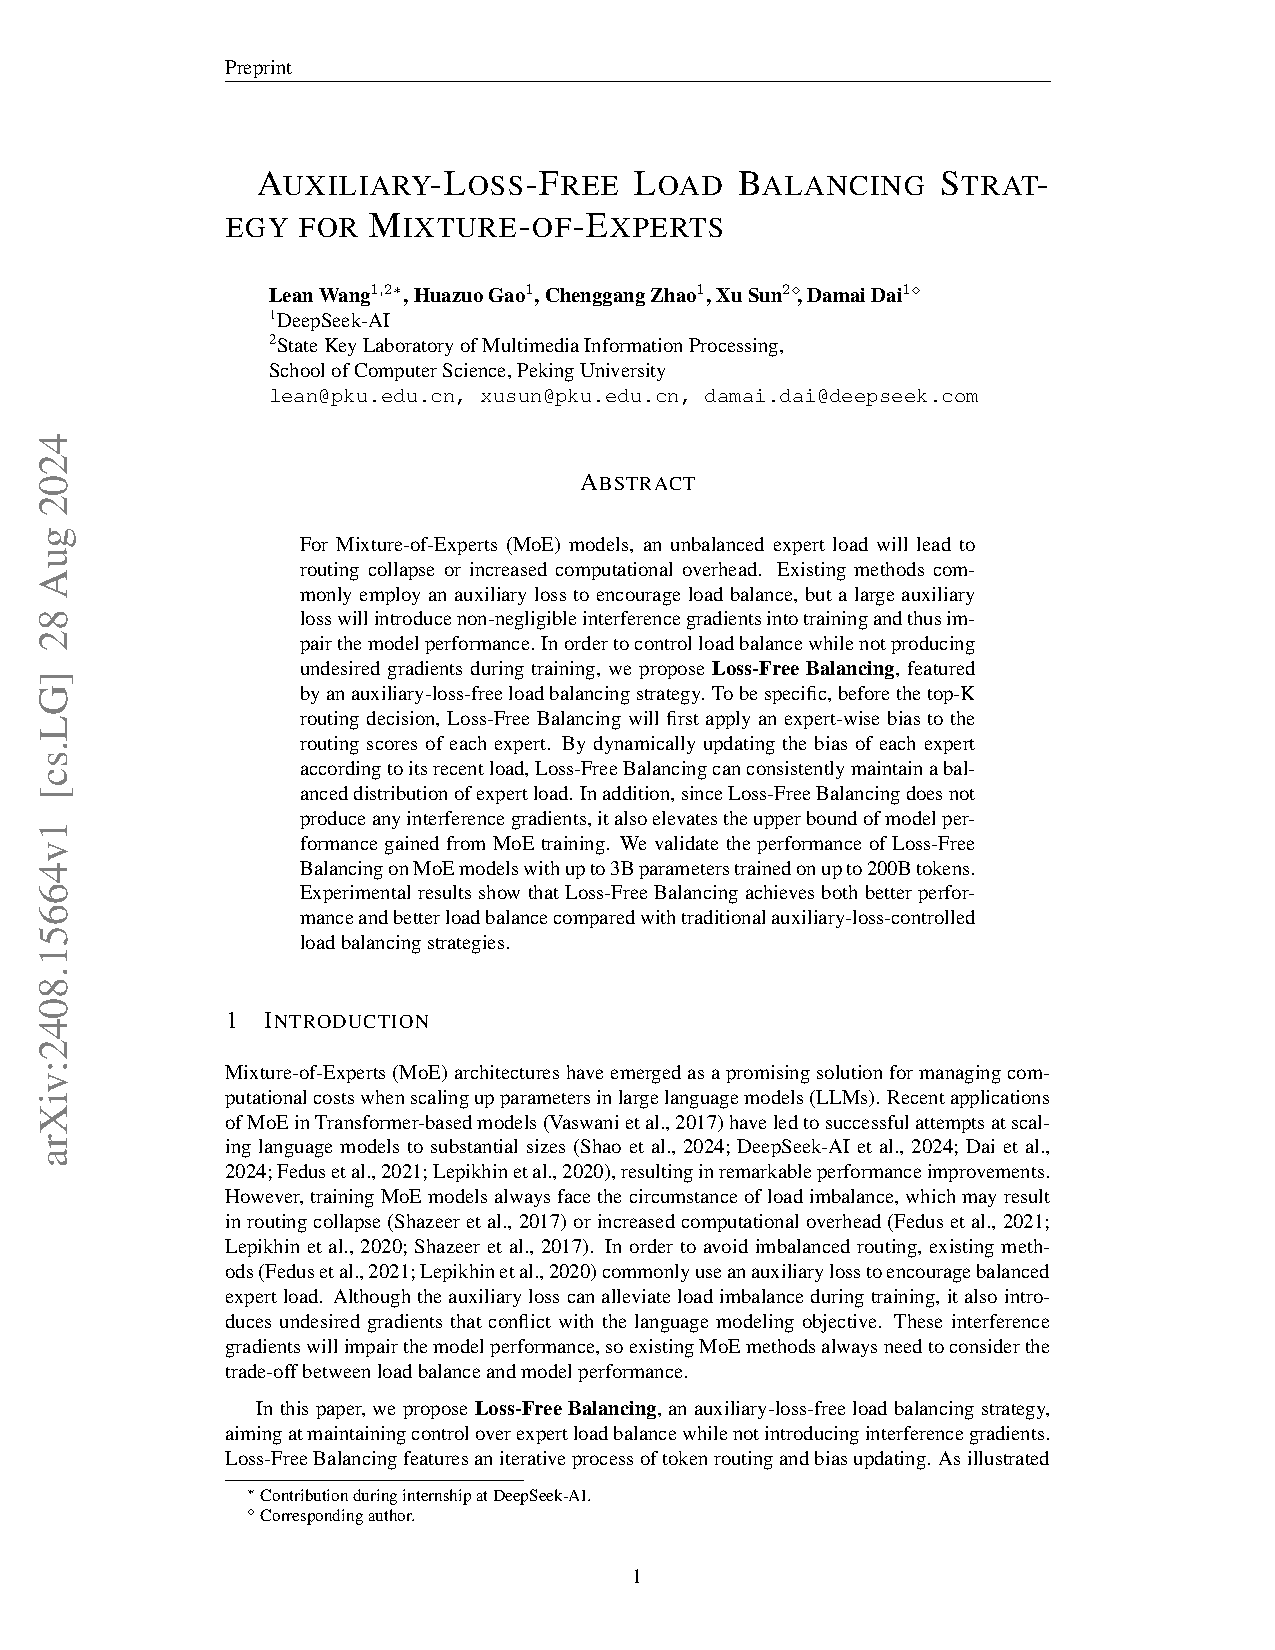
\includepdf[pages=-,pagecommand={}]{pdfs/wang-2024-auxfree.pdf}

\addcontentsline{toc}{subsection}{[2024] T\"ulu 3: Pushing Frontiers in Open Language Model Post-Training (Lambert et al.)}
\phantomsection
\label{paper:lambert-2024-tulu3}
% Paper Summary: Tulu 3: Pushing Frontiers in Open Language Model Post-Training (Lambert et al., 2024)

\begin{papersummary}{2024}{T\"ulu 3: Pushing Frontiers in Open Language Model Post-Training}{Nathan Lambert, Jacob Morrison, Valentina Pyatkin, Shengyi Huang, Hamish Ivison, et al. (Allen Institute for AI)}{T\"ulu 3 introduced reinforcement learning with verifiable rewards (RLVR) and released the complete post-training recipe---data, code, and evaluation---that turned frontier-quality alignment from a proprietary art into a reproducible procedure.}

\summaryheading{Key Ideas}
Post-training had become the least documented stage of model production: labs published weights but not the data mixtures, decontamination procedures, or optimization schedules that produced them. T\"ulu~3 documents all of it---a curated and decontaminated prompt corpus, supervised fine-tuning, preference optimization with DPO (\hyperref[paper:rafailov-2023-dpo]{Rafailov et al., 2023}), and a final stage the paper names reinforcement learning with verifiable rewards. RLVR discards the learned reward model of the RLHF pipeline (\hyperref[paper:ouyang-2022]{Ouyang et al., 2022}) in domains where correctness can be checked programmatically: a mathematics answer either matches or it does not, an instruction's constraints are either satisfied or violated. Training against these binary signals with policy-gradient methods (\hyperref[paper:schulman-2017-ppo]{Schulman et al., 2017}) yields targeted capability gains without reward-model exploitation, and the full evaluation suite is released with held-out splits to keep the recipe honest.

\summaryheading{Follow-on Works}
Verifiable rewards became the organizing idea of reasoning-era post-training. DeepSeek-R1 (\hyperref[paper:deepseek-2025-r1]{DeepSeek-AI, 2025}) drove the paradigm to its limit, training long-form reasoning purely against rule-based rewards, and the RLVR framing was adopted across open and proprietary pipelines alike, extending from mathematics and code execution to sandboxed agentic tasks with checkable end states. The released T\"ulu~3 corpus and evaluation regime became standard infrastructure for academic post-training research, and the recipe was subsequently scaled to a 405B-parameter base.

\summaryheading{Lasting Contributions}
Replacing learned preference proxies with ground-truth verification wherever the domain permits redrew the alignment landscape, concentrating preference-based techniques on the genuinely subjective remainder. Releasing a competitive post-training pipeline whole---data, code, and evaluation---restored reproducibility to the stage of the stack that had drifted furthest from published practice, and much of what is publicly known about modern post-training descends from this release.

\end{papersummary}

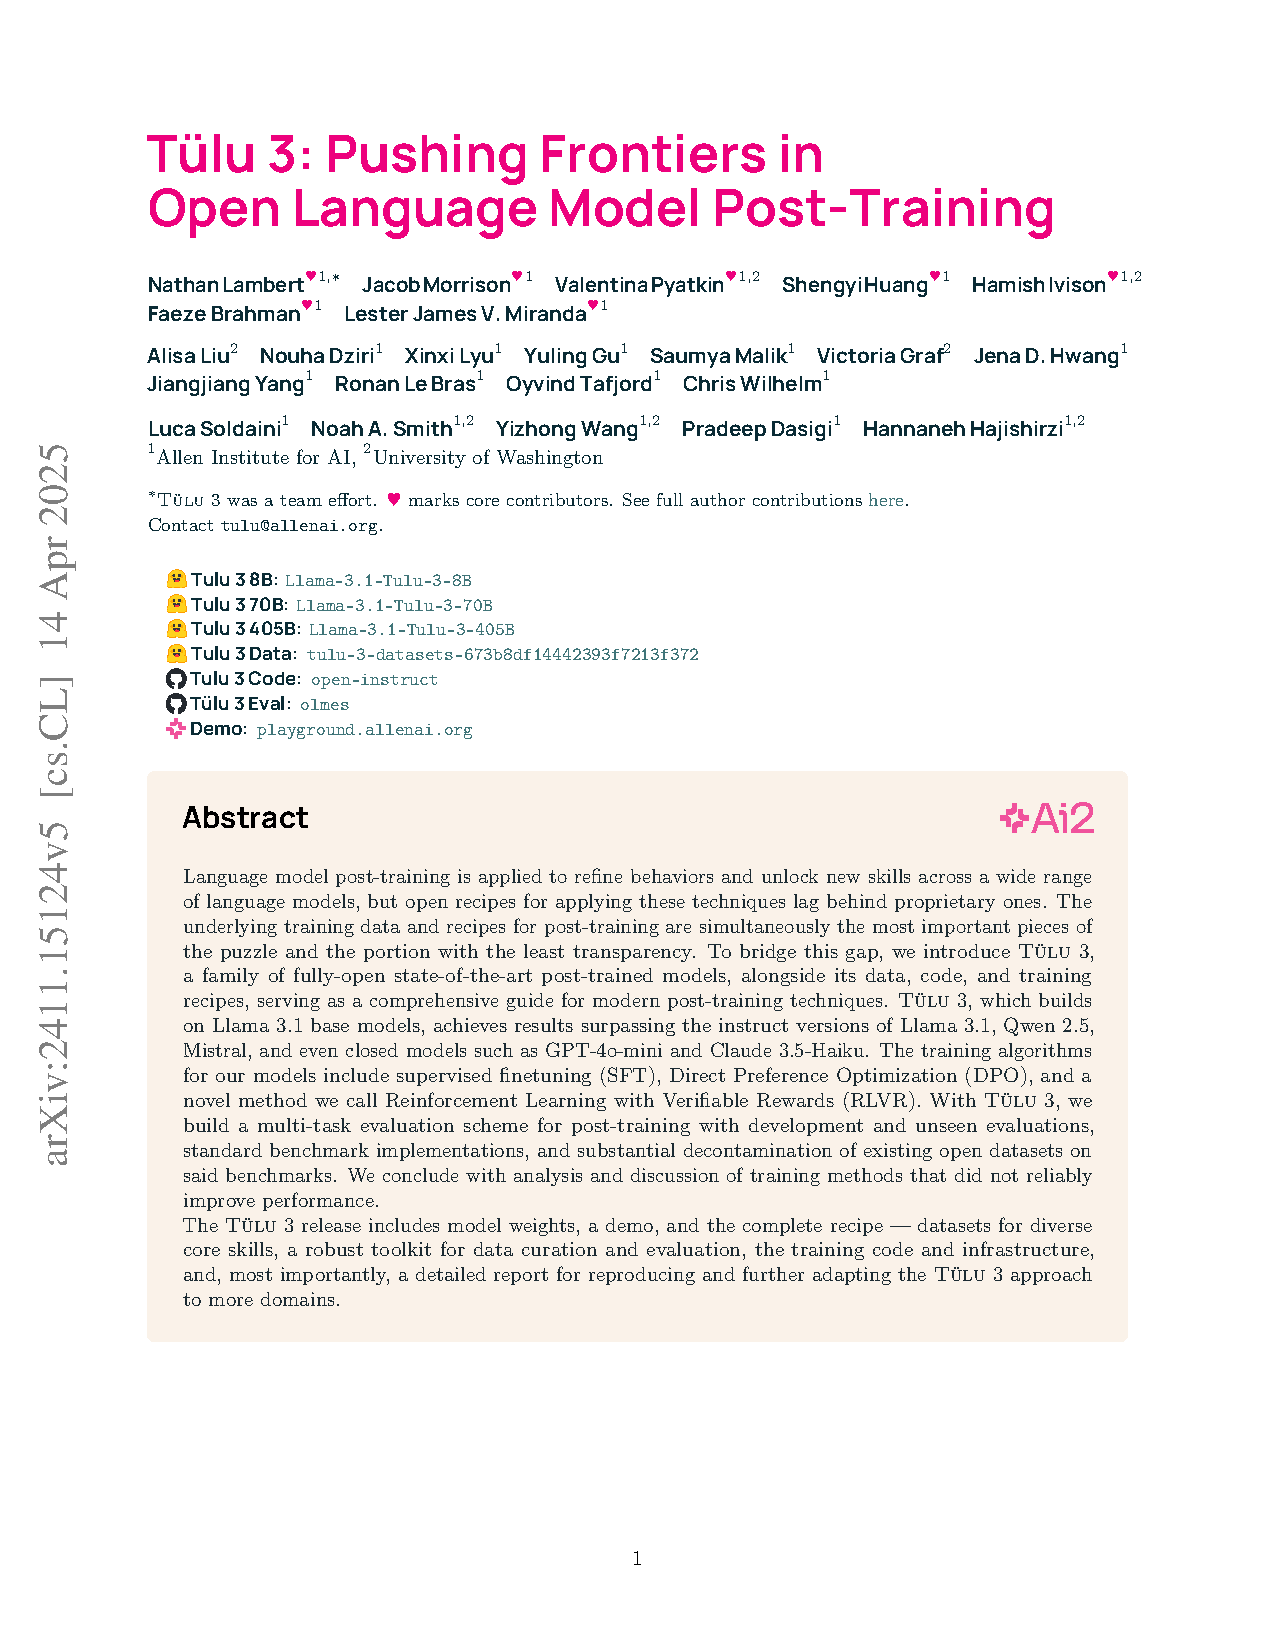
\includepdf[pages=-,pagecommand={}]{pdfs/lambert-2024-tulu3.pdf}

\addcontentsline{toc}{subsection}{[2025] DeepSeek-R1: Incentivizing Reasoning Capability in LLMs via Reinforcement Learning (DeepSeek-AI)}
\phantomsection
\label{paper:deepseek-2025-r1}
% Paper Summary: DeepSeek-R1: Incentivizing Reasoning Capability in LLMs via Reinforcement Learning (DeepSeek-AI, 2025)

\begin{papersummary}{2025}{DeepSeek-R1: Incentivizing Reasoning Capability in LLMs via Reinforcement Learning}{DeepSeek-AI (Guo et al.)}{DeepSeek-R1 demonstrated that reinforcement learning against rule-based rewards, applied directly to a base model with no supervised reasoning traces, elicits emergent chain-of-thought reasoning---and that the resulting behavior distills into small models.}

\summaryheading{Key Ideas}
The paper's central experiment, R1-Zero, applies GRPO (\hyperref[paper:shao-2024-grpo]{Shao et al., 2024}) to a base model using only mechanical rewards---answer correctness and output format---with no reward model and no demonstrations of how to reason. Over training, the model spontaneously lengthens its chain of thought (\hyperref[paper:wei-2022]{Wei et al., 2022}), and behaviors that had previously required explicit prompting or search emerge on their own: decomposition, self-verification, reflection, and mid-solution re-derivation when a path fails. The full R1 pipeline adds a small cold-start corpus, rejection sampling against the RL checkpoint, and a second reinforcement-learning stage for general helpfulness, fixing R1-Zero's readability failures while preserving its reasoning. Performance on mathematics and code matches OpenAI's o1, whose training methodology was never disclosed; R1's is documented in full, with open weights.

\summaryheading{Follow-on Works}
R1 converted the reasoning model from a proprietary artifact into a research object. Its distilled variants---small dense models fine-tuned on traces from the large one---outperformed direct RL at the same scale, establishing distillation of reasoning as standard practice. Open reproductions and refinements of its recipe (Open-Reasoner-Zero, DAPO, and successors) followed within months, verifiable-reward RL in the T\"ulu~3 sense (\hyperref[paper:lambert-2024-tulu3]{Lambert et al., 2024}) became the default post-training paradigm, and the trained-search perspective it validated connected directly to the test-time compute analysis of \hyperref[paper:snell-2024-test-time]{Snell et al.\ (2024)}. A peer-reviewed account later appeared in \textit{Nature}, a first for a frontier language model's training methodology.

\summaryheading{Lasting Contributions}
R1-Zero established that extended reasoning can be elicited from a sufficiently capable base model by outcome-based optimization alone, without demonstrations of the reasoning process. This redirected post-training work across the field toward reward design rather than trace collection, and the open release let researchers outside the originating laboratory reproduce and audit the result.

\end{papersummary}

\includepdf[pages=-,pagecommand={}]{pdfs/deepseek-2025-r1.pdf}

\addcontentsline{toc}{subsection}{[2025] Muon is Scalable for LLM Training (Liu et al.)}
\phantomsection
\label{paper:liu-2025-muon}
% Paper Summary: Muon is Scalable for LLM Training (Liu et al., 2025)

\begin{papersummary}{2025}{Muon is Scalable for LLM Training}{Jingyuan Liu, Jianlin Su, Xingcheng Yao, Zhejun Jiang, Guokun Lai, et al. (Moonshot AI)}{Muon replaces AdamW's per-coordinate scaling with approximate orthogonalization of the momentum matrix; this paper's weight-decay and update-scale corrections made it the first optimizer to show roughly twice AdamW's compute efficiency in matched scaling-law comparisons.}

\summaryheading{Key Ideas}
Adam-family optimizers (\hyperref[paper:kingma-ba-2014]{Kingma \& Ba, 2014}) treat every parameter as an independent scalar. Muon, introduced by Jordan and colleagues on small-scale benchmarks, instead treats each weight matrix as a matrix: it orthogonalizes the momentum update via a Newton--Schulz iteration, equalizing the update's singular values so that no few directions dominate a layer's change. This paper supplies what scaling required: decoupled weight decay in the style of AdamW (\hyperref[paper:loshchilov-2017-adamw]{Loshchilov \& Hutter, 2017}), without which weights and activations grow unboundedly in long runs, and a per-matrix scale correction that keeps the update's root-mean-square consistent across matrix shapes, allowing AdamW learning-rate tunings to transfer directly. Scaling-law experiments show roughly twice the computational efficiency of well-tuned AdamW, and a ZeRO-style distributed implementation keeps memory and communication overhead modest. The team validated the recipe by pretraining Moonlight, a mixture-of-experts model with 16B total and 3B activated parameters, on 5.7 trillion tokens.

\summaryheading{Follow-on Works}
Moonshot's Kimi K2 carried a stabilized variant, MuonClip, into trillion-parameter pretraining, with K3 following at yet larger scale, and other 2025--2026 open models adopted Muon-family optimizers as the efficiency margin was independently reproduced. The result revived matrix-aware optimization as a research area---spectral-norm analyses, alternative orthogonalization schemes, and second-order hybrids---after nearly a decade in which AdamW's dominance had made optimizer research appear closed.

\summaryheading{Lasting Contributions}
Muon is the third optimizer generation represented in this collection: gradient descent gave way to adaptive per-coordinate methods, and Muon shows the gains available from treating each weight matrix as a matrix rather than a collection of independent scalars. A twofold efficiency improvement compounds over every training run that adopts it. The paper's insistence on controlled scaling-law comparison, matching AdamW at equal compute rather than equal steps, also set the evidentiary standard by which subsequent optimizer claims are judged.

\end{papersummary}

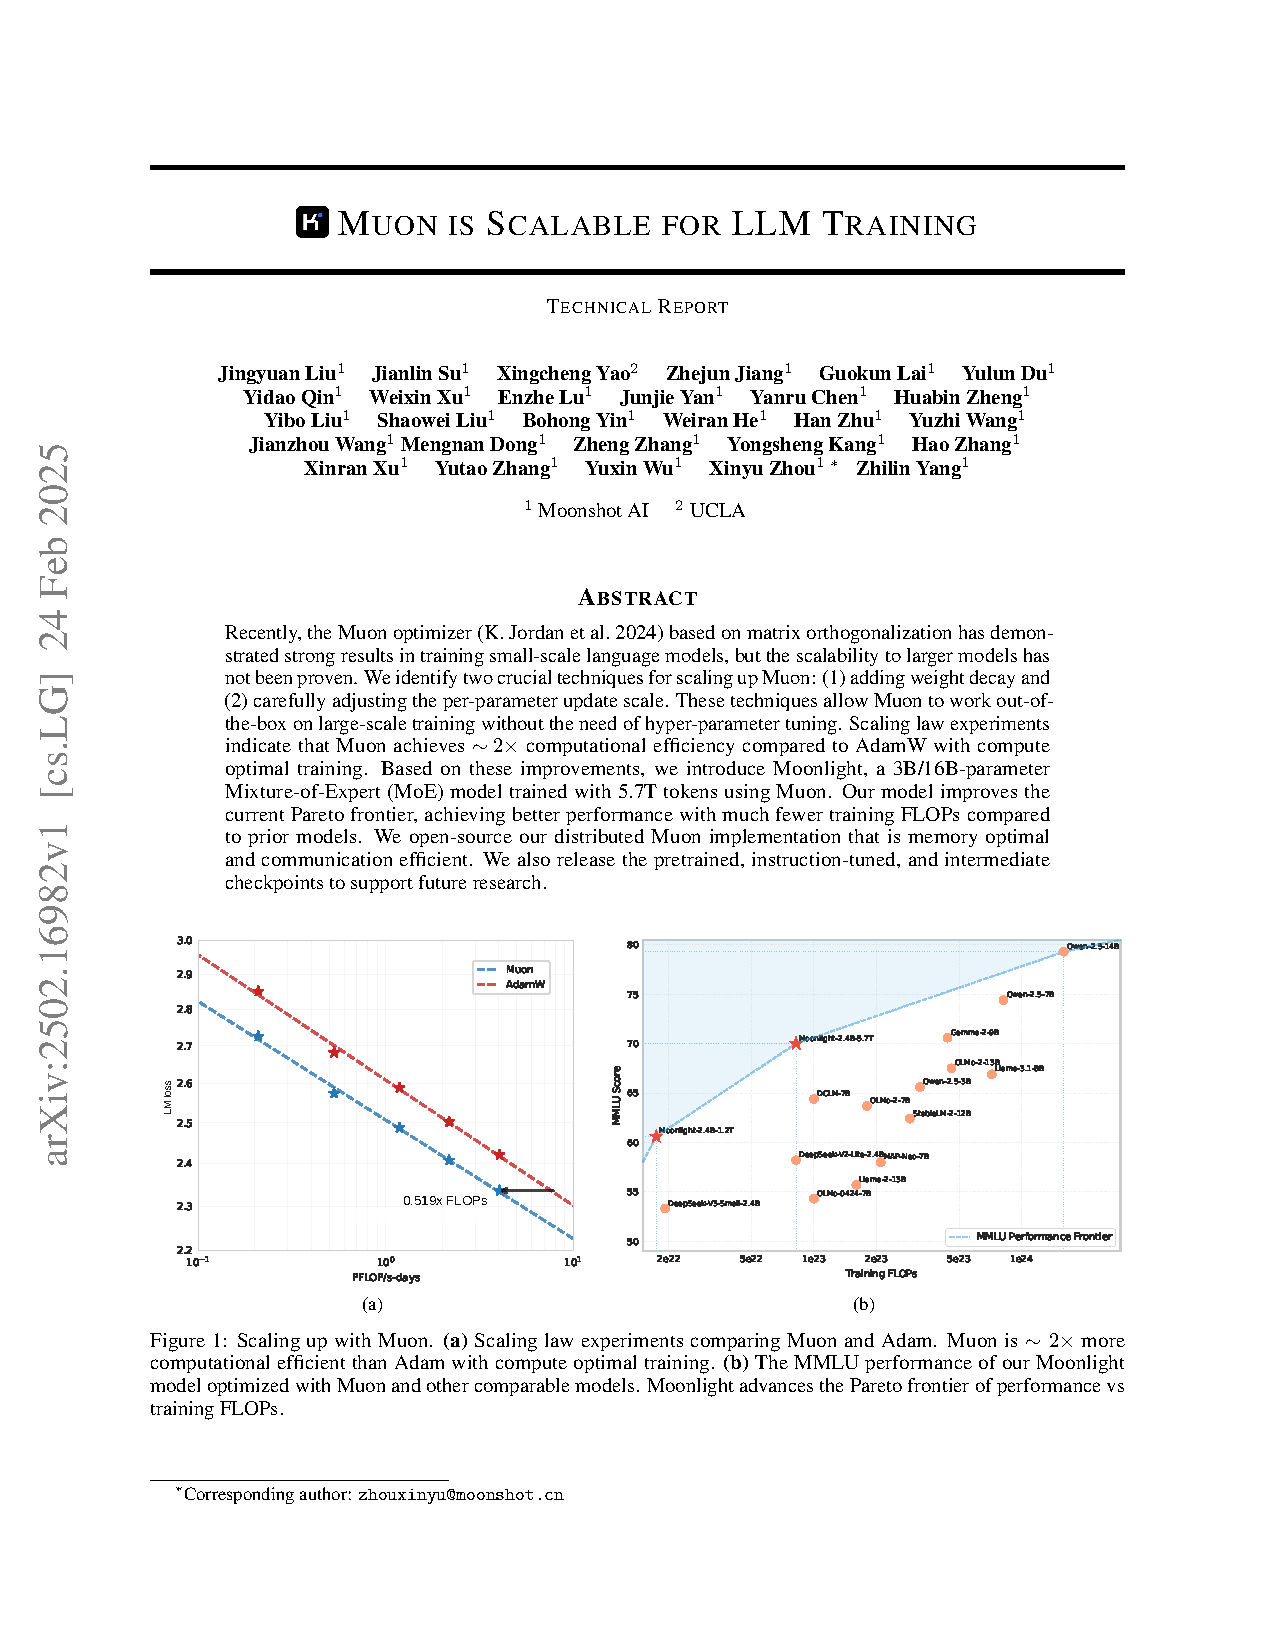
\includepdf[pages=-,pagecommand={}]{pdfs/liu-2025-muon.pdf}

\addcontentsline{toc}{subsection}{[2025] Kimi Linear: An Expressive, Efficient Attention Architecture (Kimi Team)}
\phantomsection
\label{paper:kimi-2025-linear}
% Paper Summary: Kimi Linear: An Expressive, Efficient Attention Architecture (Kimi Team, 2025)

\begin{papersummary}{2025}{Kimi Linear: An Expressive, Efficient Attention Architecture}{Kimi Team}{Kimi Delta Attention, a fine-grained gated delta rule interleaved with periodic full-attention layers, produced the first hybrid linear-attention architecture to outperform full attention under matched comparisons, at a fraction of its memory and decoding cost.}

\summaryheading{Key Ideas}
Linear attention maintains a fixed-size recurrent state instead of a growing key-value cache, but had always paid for constant-cost inference with degraded quality. Kimi Delta Attention (KDA) closes the gap by refining the delta-rule family of fast-weight updates: where prior gated variants forget with a single scalar per head, KDA gates each feature channel independently, giving the state fine-grained control over what to retain and what to overwrite, with a chunkwise algorithm engineered for high hardware utilization. The architecture interleaves three KDA layers with one full-attention layer---the periodic global layers supplying exact retrieval that recurrent state cannot guarantee, using multi-head latent attention (\hyperref[paper:deepseek-2024-v2]{DeepSeek-AI, 2024}) with no position encoding, KDA itself carrying the positional signal. Trained as a 48B-parameter mixture-of-experts model with 3B active, the hybrid outperforms a full-attention baseline under matched training while cutting key-value cache by up to 75\% and reaching roughly sixfold decoding throughput at million-token context.

\summaryheading{Follow-on Works}
Kimi K3 deployed KDA hybrids at frontier scale---2.8T parameters with native million-token context---demonstrating that the design survives the transition from controlled experiment to flagship production model, and hybrid linear-attention layouts became a standard option in subsequent open architectures. The work vindicated the research programs it builds on: the selective state-space line of Mamba (\hyperref[paper:gu-dao-2023]{Gu \& Dao, 2023}), the trainable sparsity of NSA (\hyperref[paper:yuan-2025-nsa]{Yuan et al., 2025}), and the gating analyses of \hyperref[paper:qiu-2025-gated-attention]{Qiu et al.\ (2025)}, whose mechanisms KDA generalizes to the fast-weight setting.

\summaryheading{Lasting Contributions}
For eight years after the transformer, quadratic attention was the price of quality; this paper broke that equivalence with a hybrid that improved on full attention while reducing both memory and decoding cost. It also reframed the practical long-context question as how sparsely the exact-retrieval layers can be placed, rather than whether recurrence can replace attention outright, and its channel-wise gating established the delta rule, a lineage reaching back to fast-weight programming, as a standard component of frontier model architecture.

\end{papersummary}

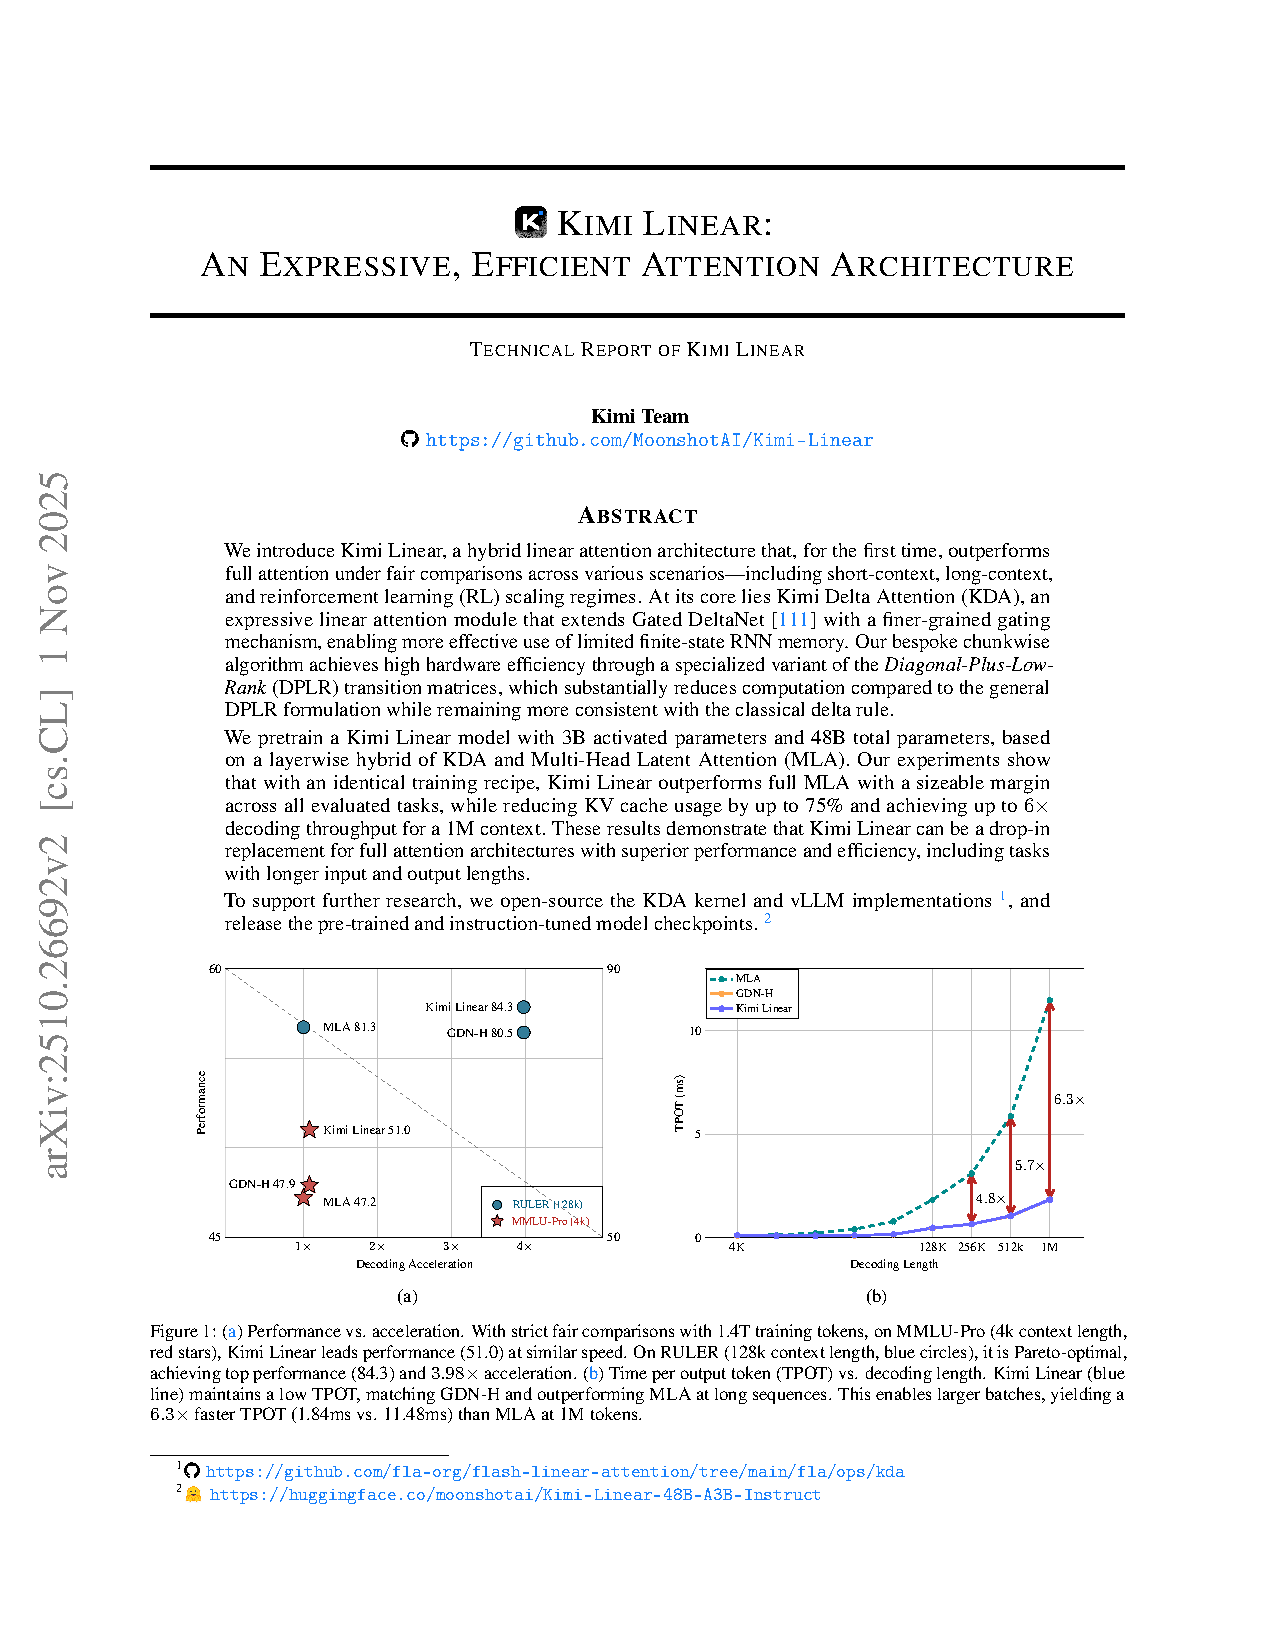
\includepdf[pages=-,pagecommand={}]{pdfs/kimi-2025-linear.pdf}

\addcontentsline{toc}{subsection}{[2026] LatentMoE: Toward Optimal Accuracy per FLOP and Parameter in Mixture of Experts (Elango et al.)}
\phantomsection
\label{paper:elango-2026-latentmoe}
% Paper Summary: LatentMoE: Toward Optimal Accuracy per FLOP and Parameter in Mixture of Experts (Elango et al., 2026)

\begin{papersummary}{2026}{LatentMoE: Toward Optimal Accuracy per FLOP and Parameter in Mixture of Experts}{Venmugil Elango, Nidhi Bhatia, Roger Waleffe, Rasoul Shafipour, Tomer Asida, et al. (NVIDIA)}{LatentMoE routes compressed latent representations to experts rather than full hidden states, redesigning the mixture-of-experts layer around accuracy per FLOP and per parameter from a hardware--software co-design perspective.}

\summaryheading{Key Ideas}
Mixture-of-experts architectures (\hyperref[paper:shazeer-2017-moe]{Shazeer et al., 2017}) decouple capacity from per-token compute, but the paper asks the sharper question of how close existing designs are to optimal per unit of inference cost. Characterizing bottlenecks across deployment regimes---compute-bound prefill, bandwidth-bound decode, memory-capacity-bound serving---it finds that expert layers operating on the full hidden dimension spend FLOPs, parameters, and memory traffic that better placement could avoid. LatentMoE inserts a learned down-projection so that routing and expert computation occur in a compressed latent space, with expansion following afterward: the same architectural move that multi-head latent attention (\hyperref[paper:deepseek-2024-v2]{DeepSeek-AI, 2024}) applied to the key-value cache, applied here to conditional computation. The savings are reinvested: total expert count and the number of experts active per token rise by the compression factor, so capacity grows at roughly unchanged inference cost. A design-space exploration up to 95B parameters over a 1-trillion-token training horizon shows the layout dominating standard fine-grained mixture-of-experts designs on accuracy per FLOP and per parameter, and the design composes with feedback-based load balancing (\hyperref[paper:wang-2024-auxfree]{Wang et al., 2024}).

\summaryheading{Follow-on Works}
NVIDIA's flagship Nemotron-3 Super and Ultra models adopted the architecture and scaled it substantially, and Kimi K3's stabilized variant---896 routed experts with 16 active per token---carried latent expert routing into the largest open model of its time, adding quantile-based balancing for stability at that width. Published in January 2026, it is the most recent paper in this collection, adopted by two independent frontier families within months of release; its framing complements the compute-optimal analyses of mixture-of-experts scaling begun by \hyperref[paper:krajewski-2024]{Krajewski et al.\ (2024)}.

\summaryheading{Lasting Contributions}
The paper reframes sparse-layer design as explicit optimization of accuracy per unit of deployed resource rather than parameter count, a framing aligned with an era in which inference rather than training dominates the cost of a model's life. Latent-space conditional computation extends the compression lineage running through this volume, from low-rank adaptation to latent attention, to the expert layer itself.

\end{papersummary}

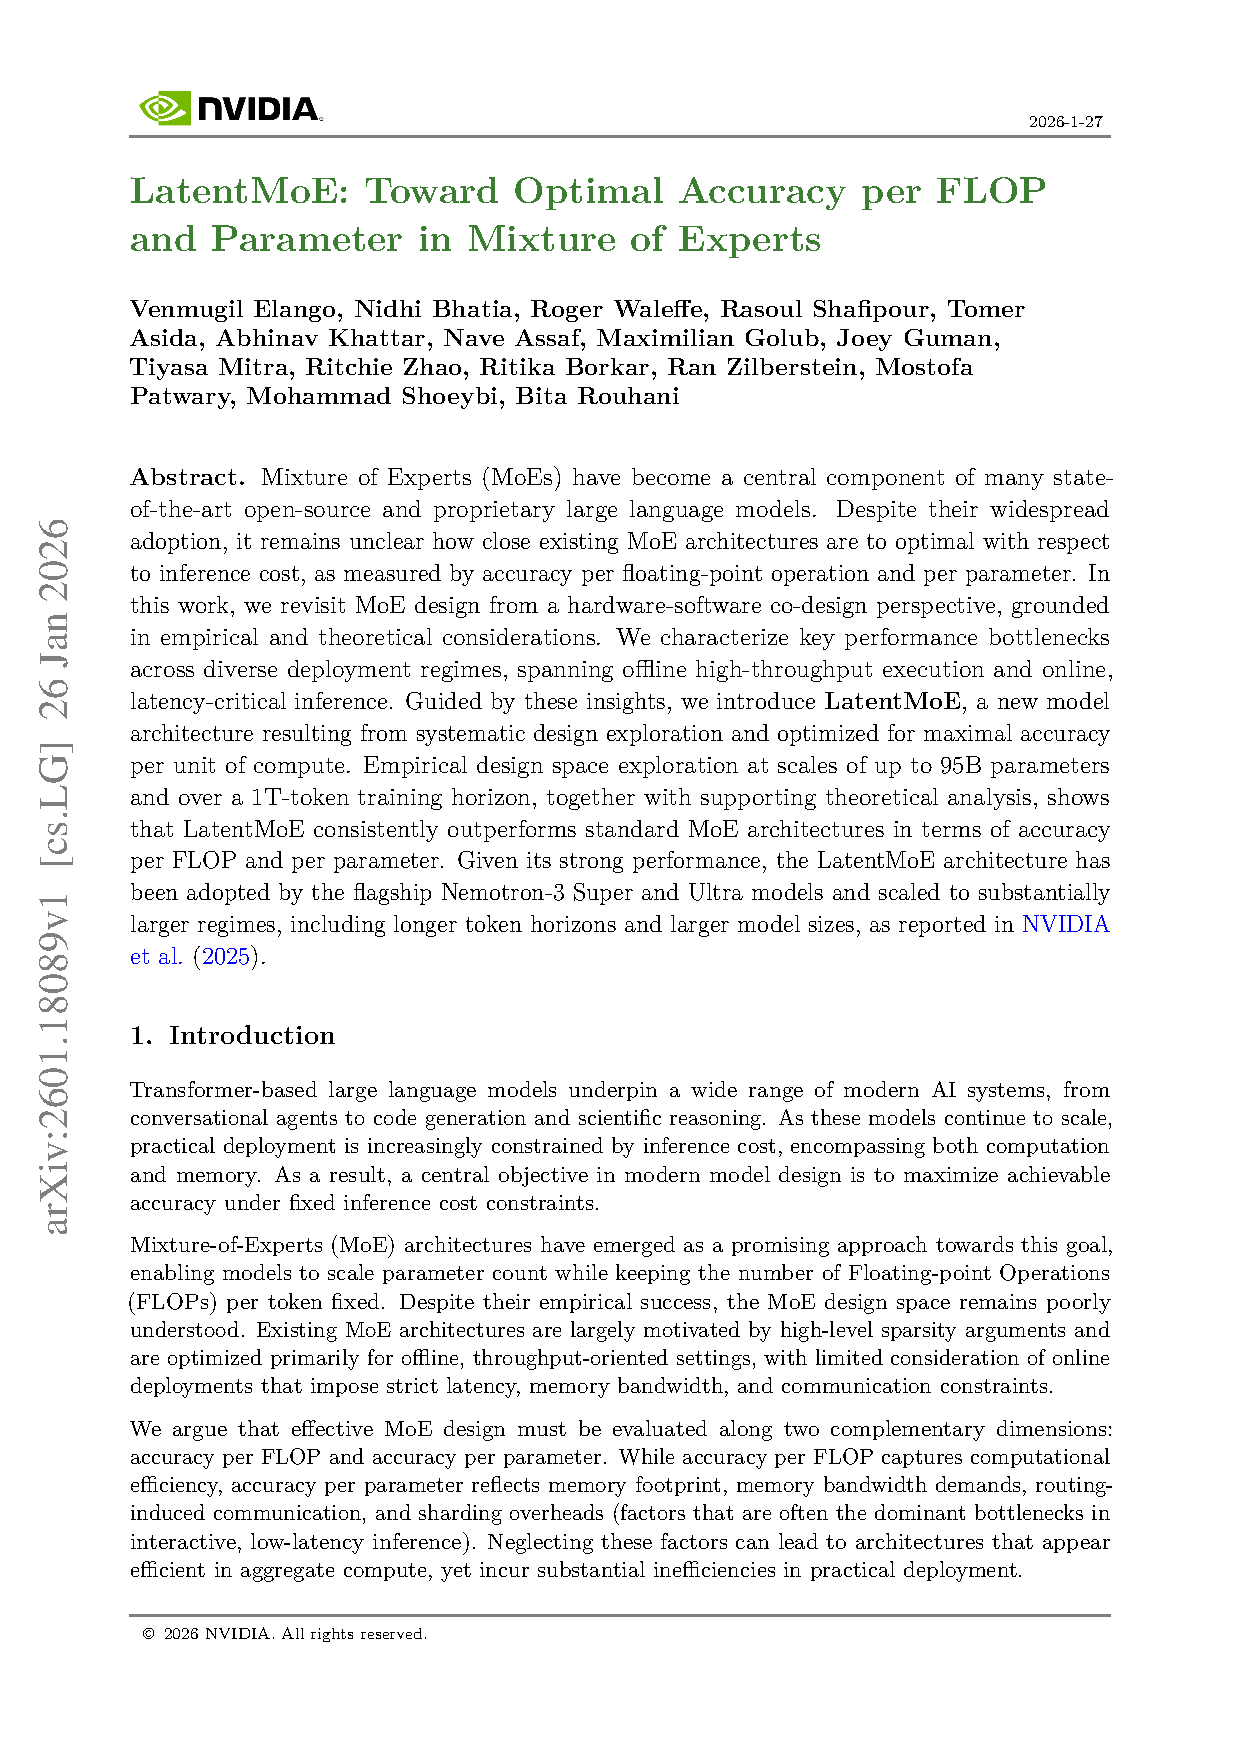
\includepdf[pages=-,pagecommand={}]{pdfs/elango-2026-latentmoe.pdf}



% Appendices — styled as parts so they appear at the same level in the TOC
\appendix
\setcounter{part}{0}
\renewcommand{\thepart}{\Alph{part}}
\renewcommand{\theHpart}{appendix.\Alph{part}}
\renewcommand{\partname}{Appendix}

% Appendix A: Emerging Results (2023–2025)
\part[Emerging Results]{Emerging Results\texorpdfstring{\\}{, }2023--2025}
\input{content/appendix-a-chapter}

% Appendix B: Foundations of Agents (2022–2025)
\part[Foundations of Agents]{Foundations of Agents\texorpdfstring{\\}{, }2022--2025}
\input{content/appendix-b-chapter}

% Back matter
\backmatter

% Epilogue
\input{content/epilogue}

% Index
% \printindex forces its own page break internally (via theindex's
% \twocolumn), so the TOC anchor must be created after that break --
% patching \@makeschapterhead is the only hook point inside \twocolumn's
% optional argument, which runs after the break. Adding it before, as an
% ordinary \addcontentsline preceding \printindex, would (as with the
% papersummary anchors, fixed earlier) bind "Index" to whatever page was
% current before the break rather than the index's actual first page.
{%
  \makeatletter
  \let\org@makeschapterhead\@makeschapterhead
  \def\@makeschapterhead#1{%
    \org@makeschapterhead{#1}%
    \phantomsection
    \addcontentsline{toc}{chapter}{#1}%
  }%
  \makeatother
  \printindex
}

\end{document}